\chapter{Parked data trigger efficiencies}
\label{app:trigeffs}
This appendix contains the trigger efficiency curves with overlaid error function fits and there errors as described in \SectionRef{sec:parkedtrigger}. Due to the event selection applied in the parked data analysis only the highest bin in \Mjj is used.

\begin{figure}[h!]
  \begin{center}
    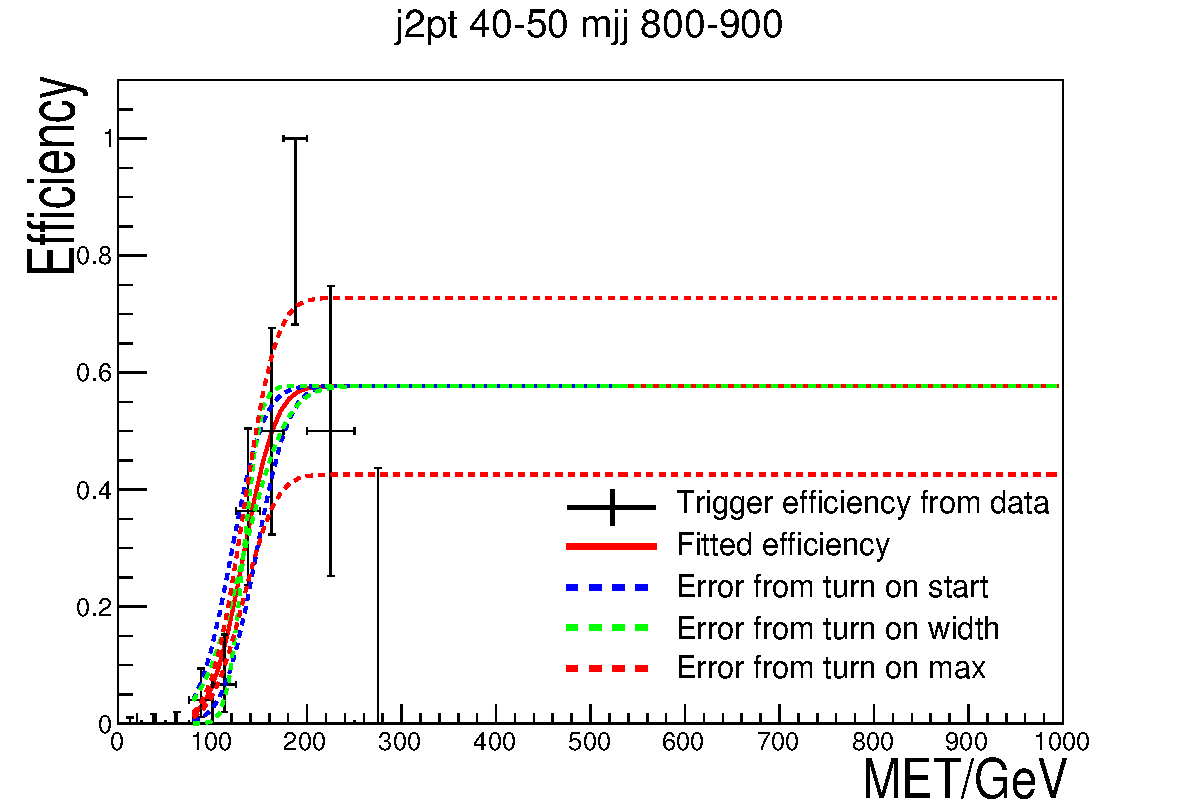
\includegraphics[width=.6\largefigwidth]{plots/parked/trigfitplots/hData_MET_1D_23A.pdf}
    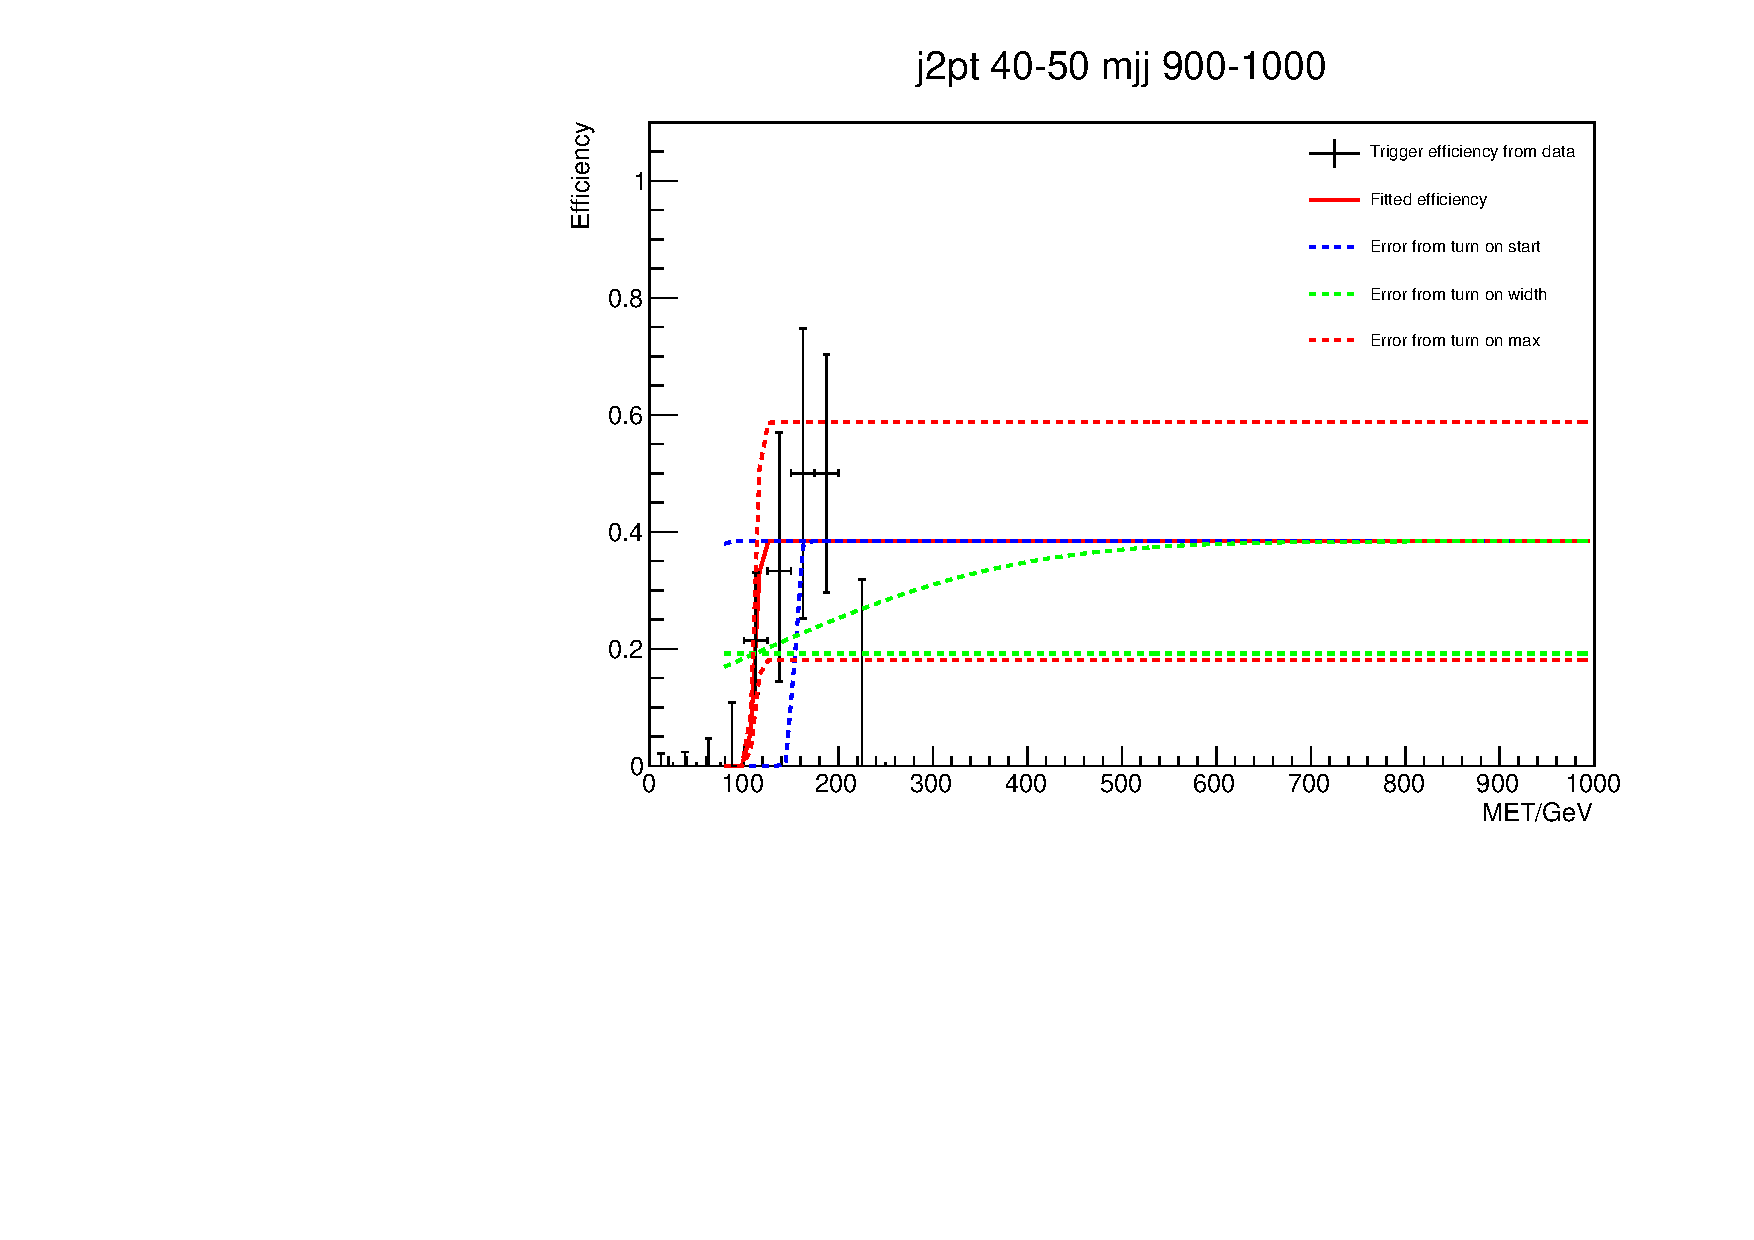
\includegraphics[width=.6\largefigwidth]{plots/parked/trigfitplots/hData_MET_1D_24A.pdf}

    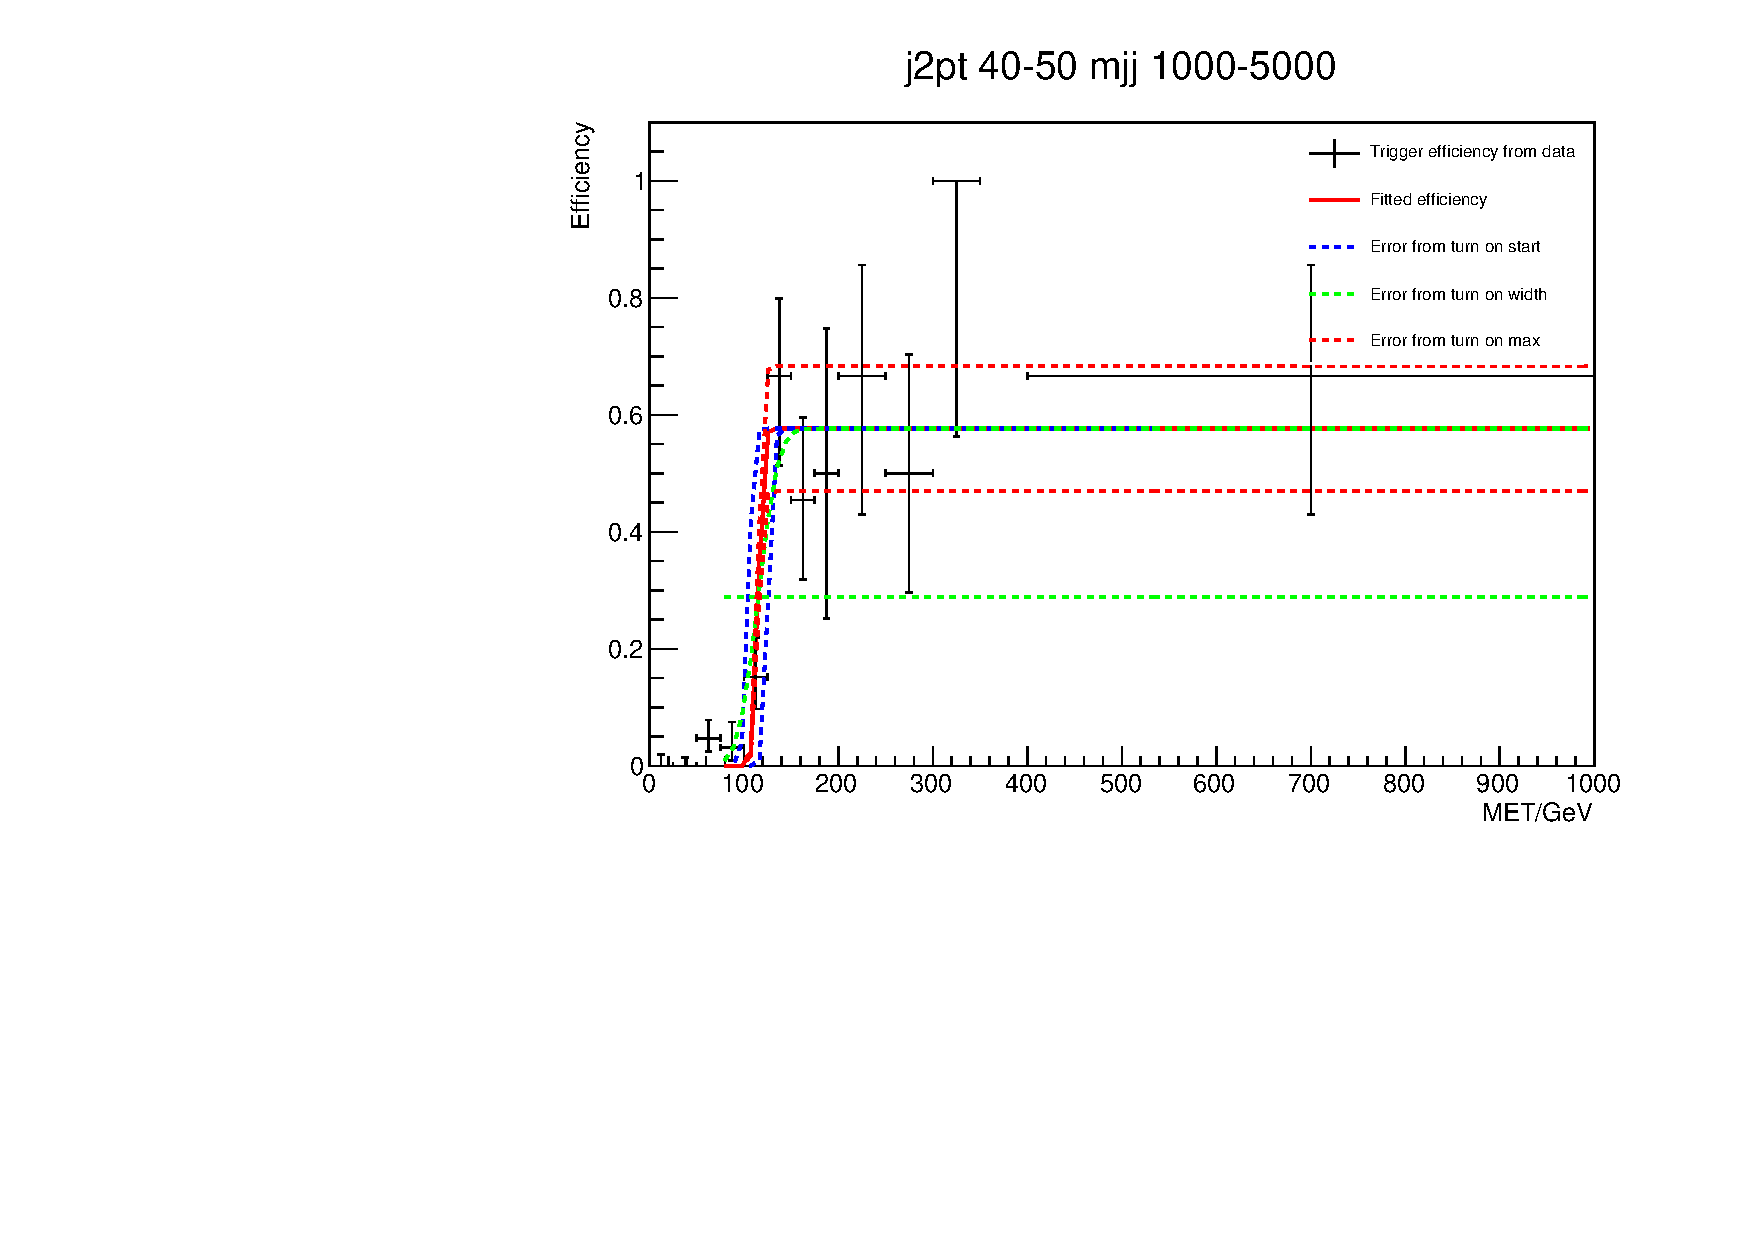
\includegraphics[width=.6\largefigwidth]{plots/parked/trigfitplots/hData_MET_1D_25A.pdf}
    \caption{The measured efficiency of the trigger used in run A as a function of MET in bins of dijet mass (mjj) and sub-leading jet $p_{T}$ (j2pt). The bin that each plot corresponds to is displayed at the top of the plot}
    \label{fig:trigfitplotsA1}
  \end{center}
\end{figure}

\begin{figure}[h!]
  \begin{center}
    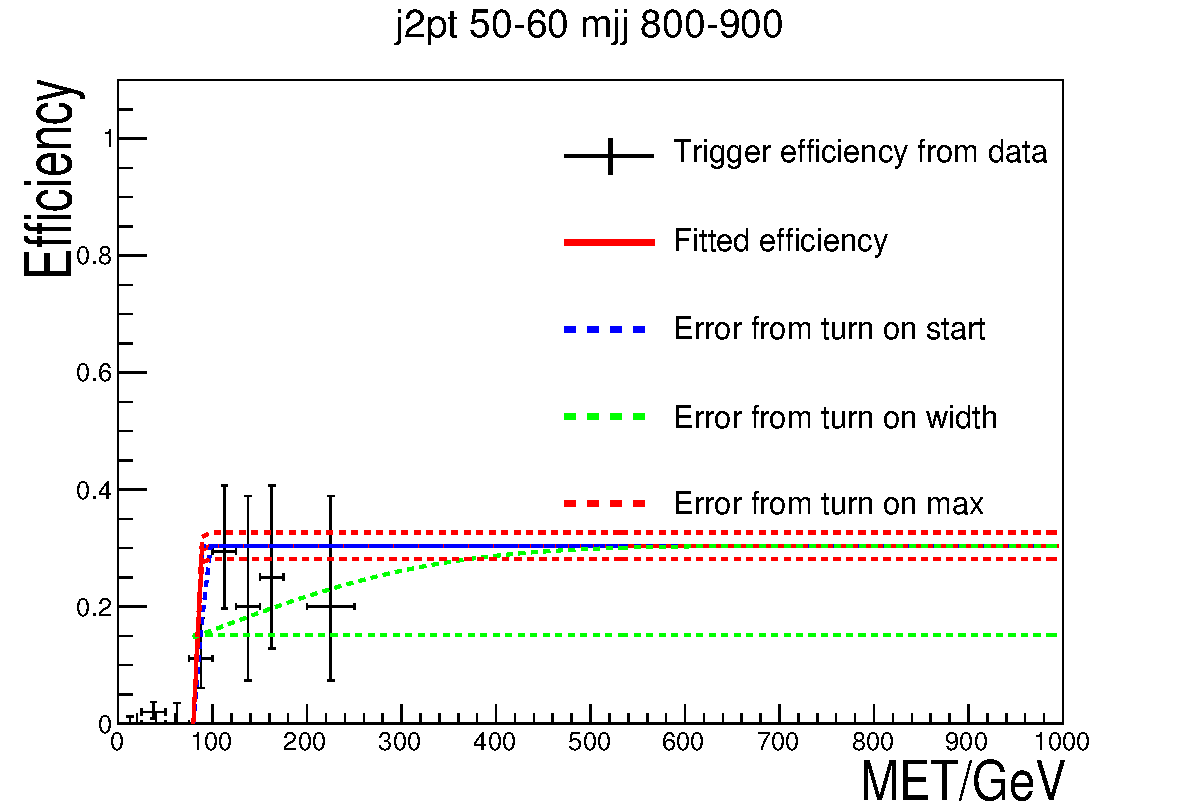
\includegraphics[width=.6\largefigwidth]{plots/parked/trigfitplots/hData_MET_1D_33A.pdf}
    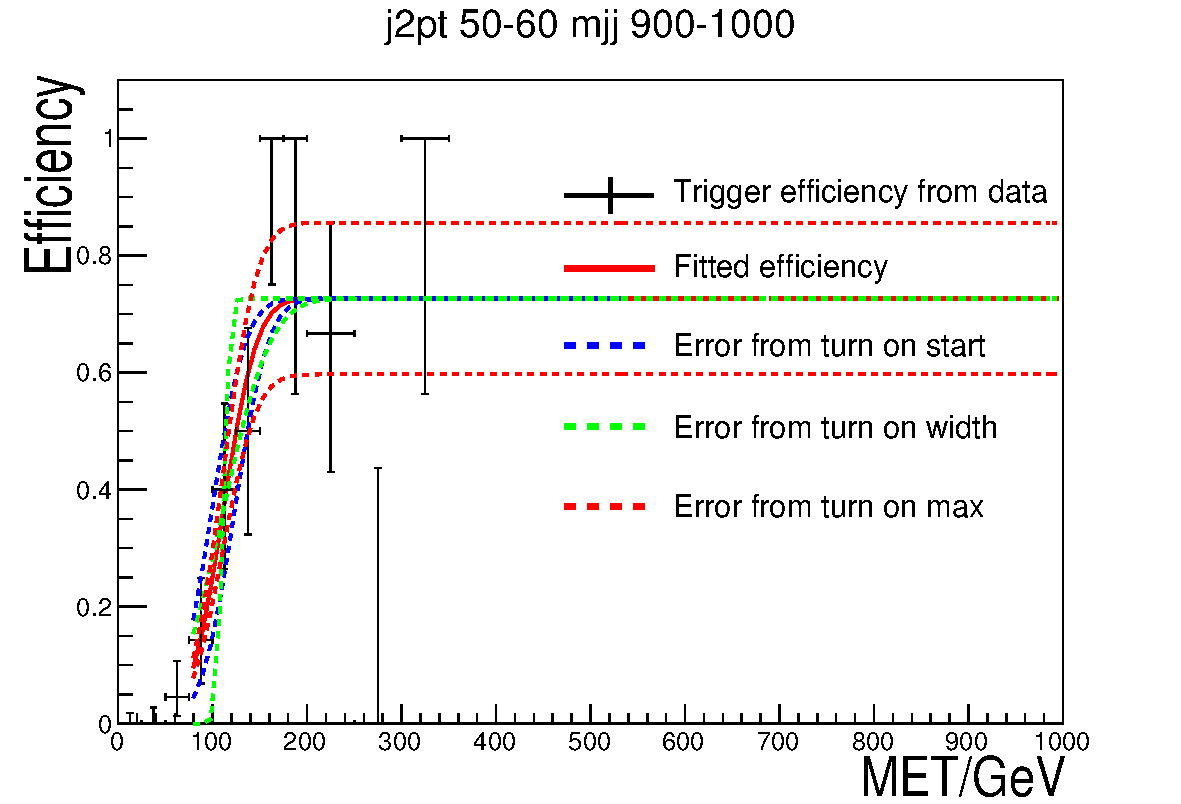
\includegraphics[width=.6\largefigwidth]{plots/parked/trigfitplots/hData_MET_1D_34A.pdf}

    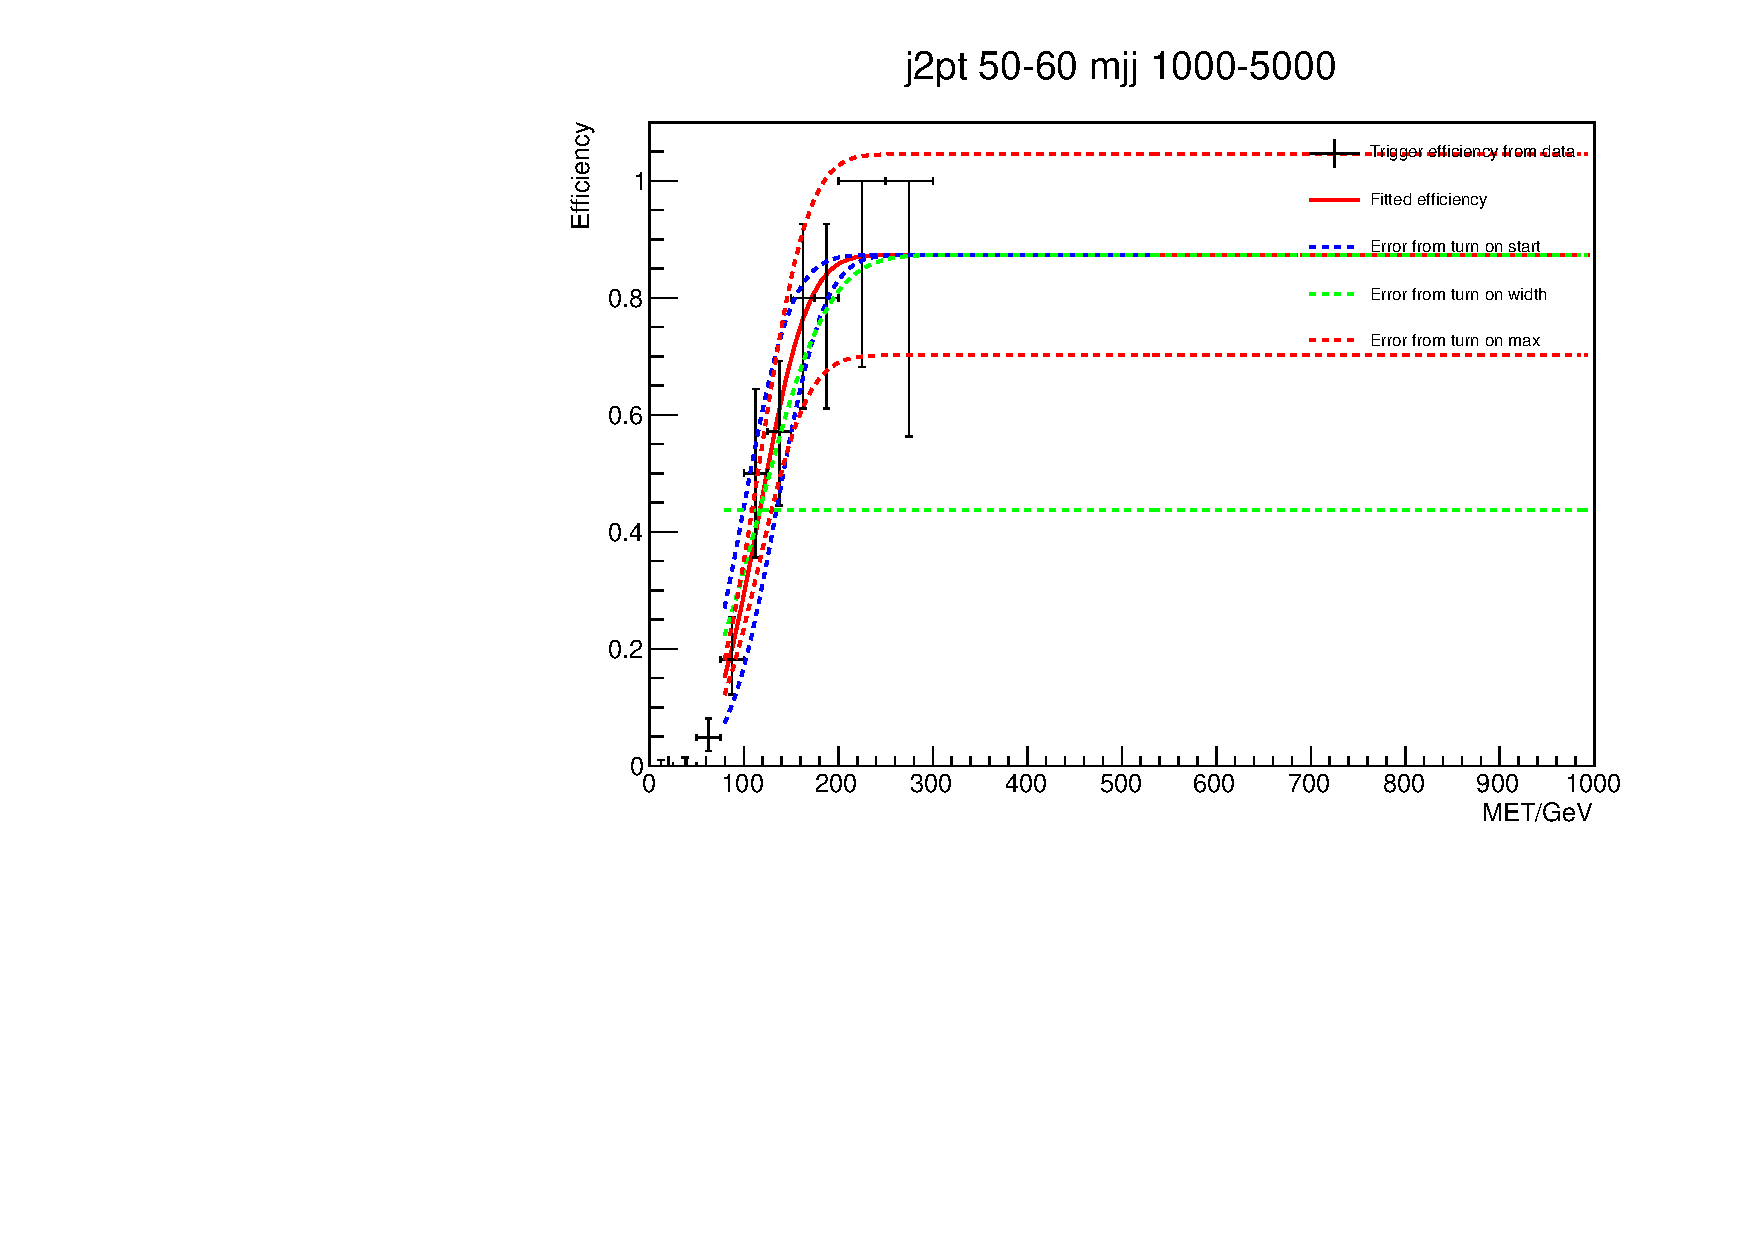
\includegraphics[width=.6\largefigwidth]{plots/parked/trigfitplots/hData_MET_1D_35A.pdf}
    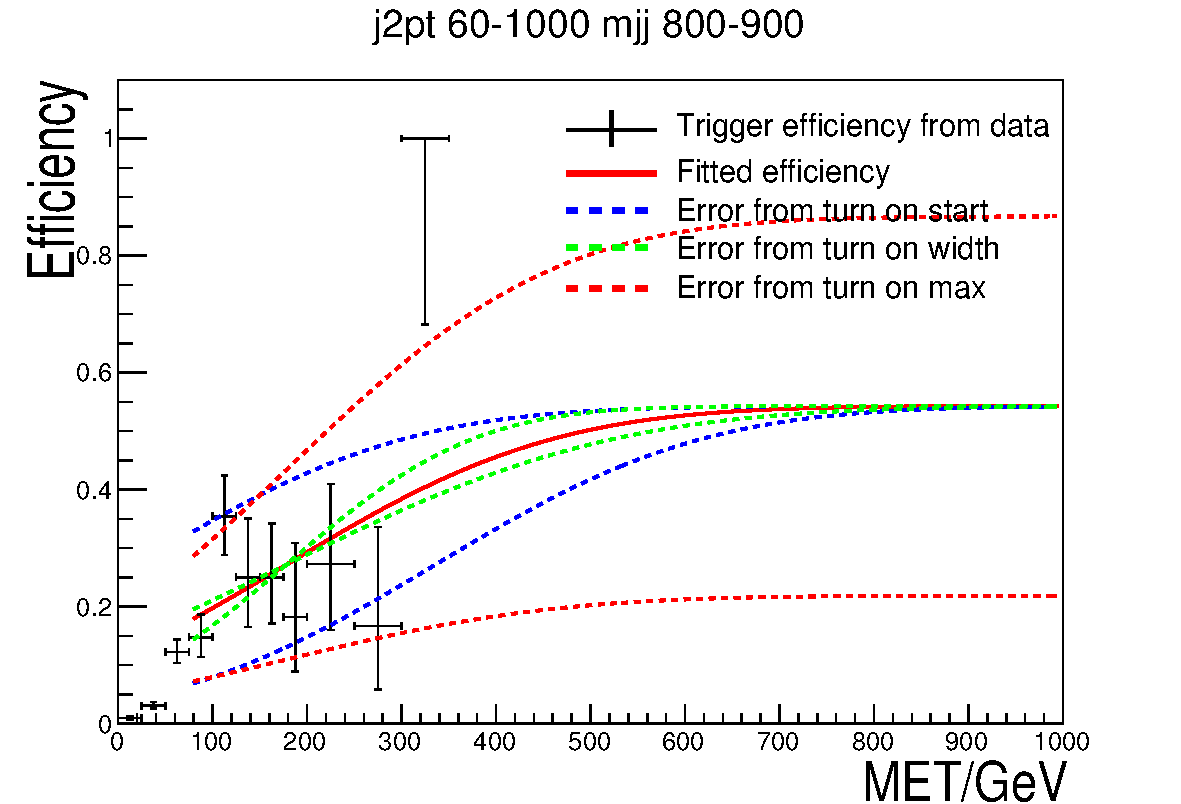
\includegraphics[width=.6\largefigwidth]{plots/parked/trigfitplots/hData_MET_1D_43A.pdf}

    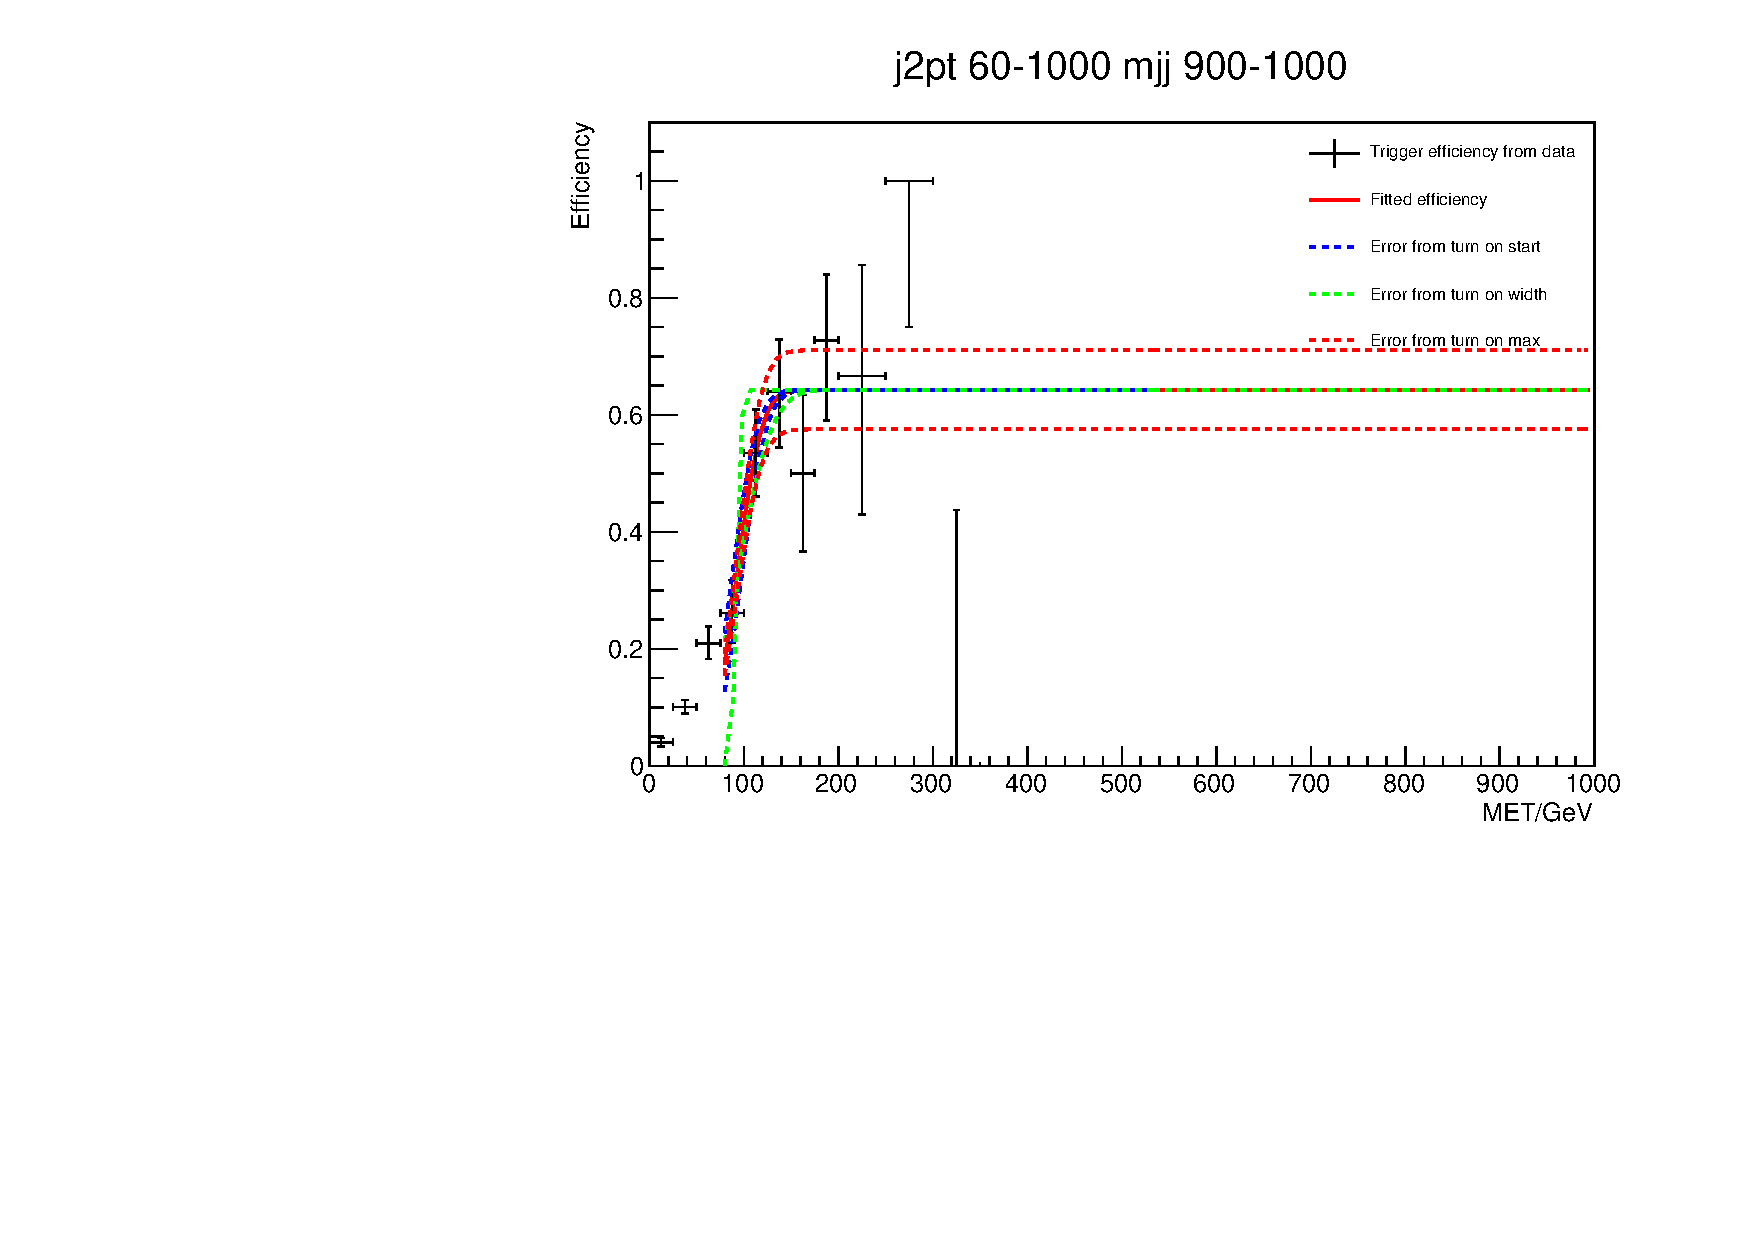
\includegraphics[width=.6\largefigwidth]{plots/parked/trigfitplots/hData_MET_1D_44A.pdf}
    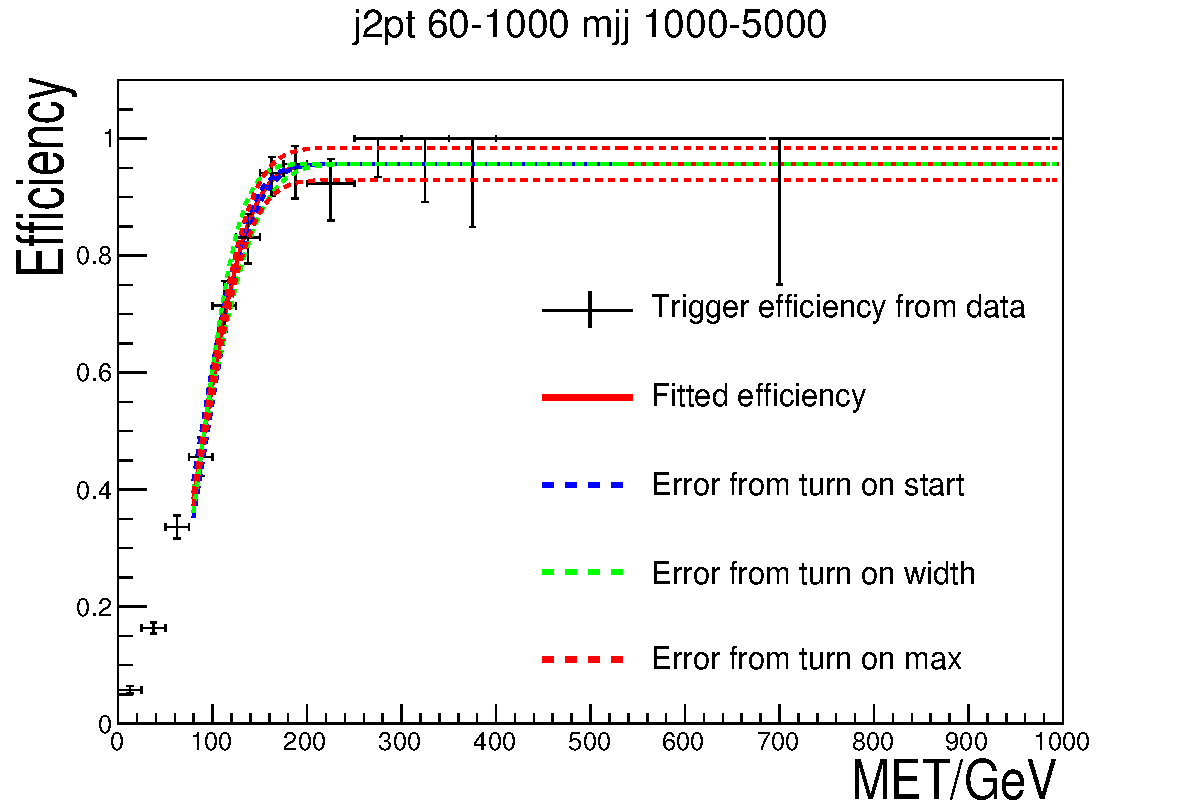
\includegraphics[width=.6\largefigwidth]{plots/parked/trigfitplots/hData_MET_1D_45A.pdf}
    \caption{The measured efficiency of the trigger used in run A as a function of MET in bins of dijet mass (mjj) and sub-leading jet $p_{T}$ (j2pt). The bin that each plot corresponds to is displayed at the top of the plot}
    \label{fig:trigfitplotsA2}
  \end{center}
\end{figure}

\begin{figure}[h!]
  \begin{center}
    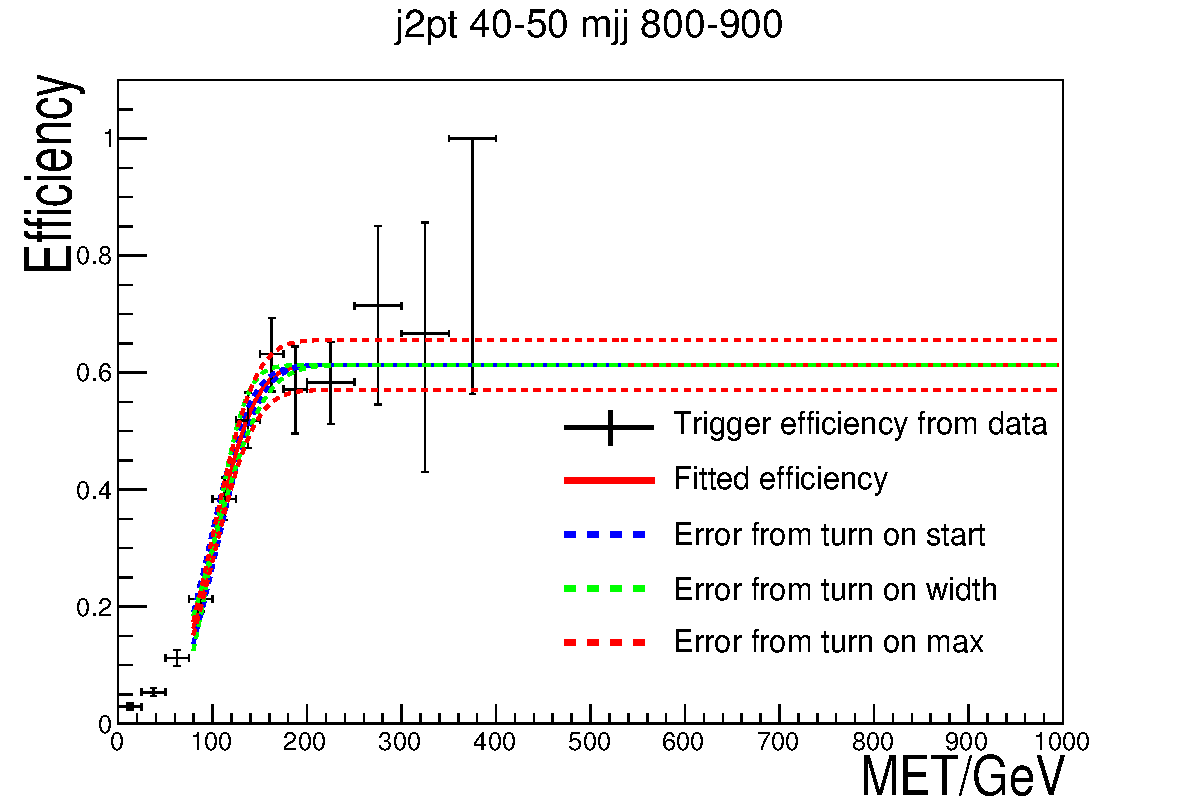
\includegraphics[width=.6\largefigwidth]{plots/parked/trigfitplots/hData_MET_1D_23BC.pdf}
    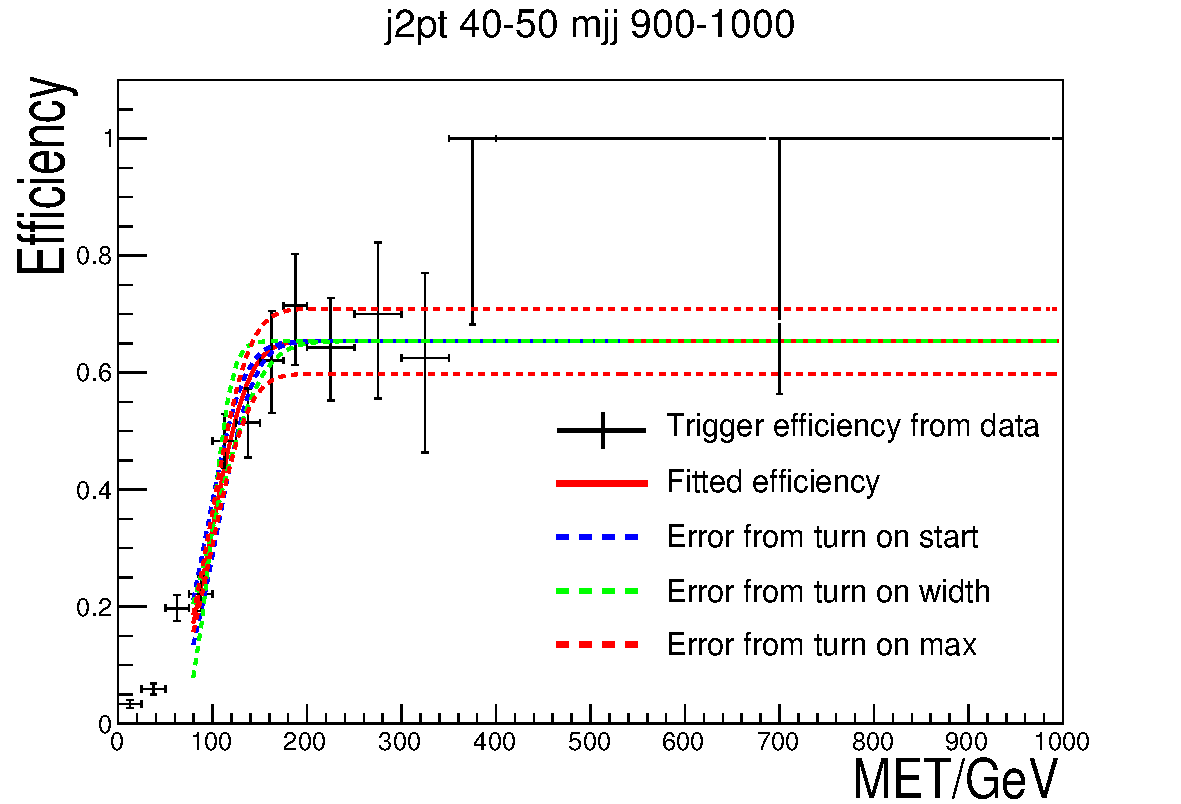
\includegraphics[width=.6\largefigwidth]{plots/parked/trigfitplots/hData_MET_1D_24BC.pdf}

    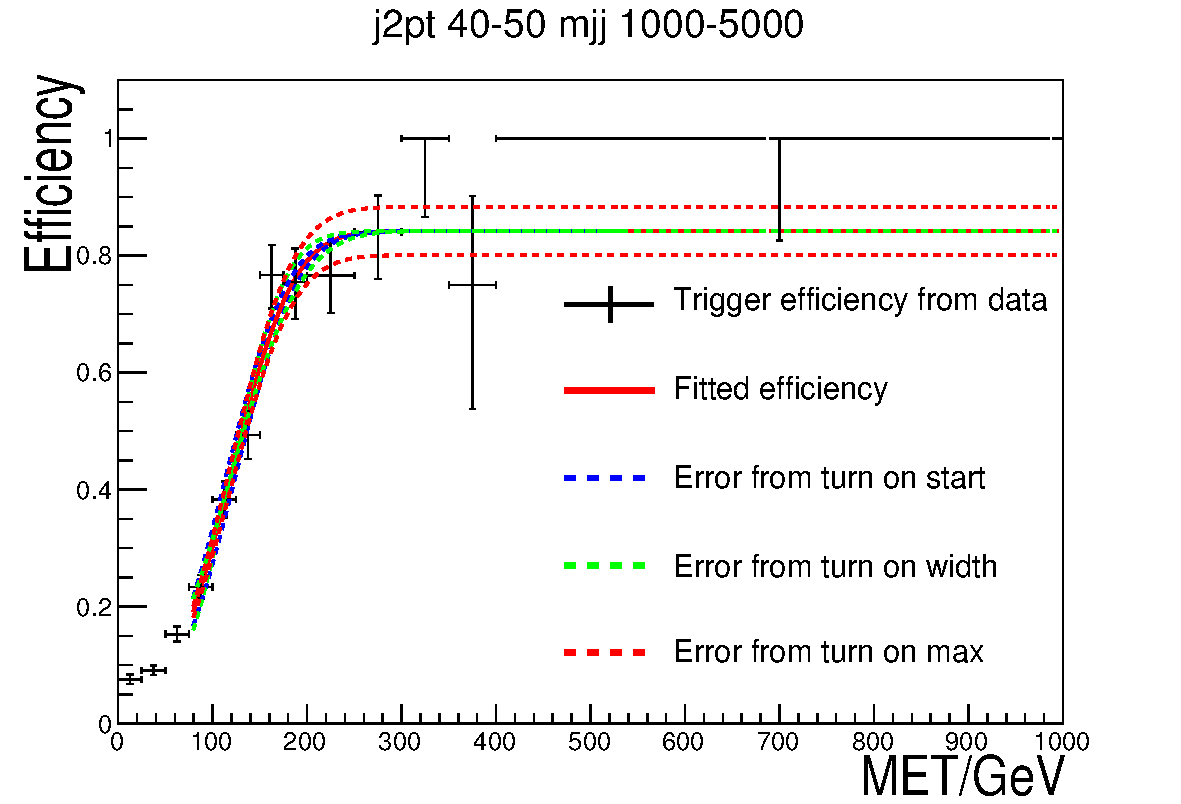
\includegraphics[width=.6\largefigwidth]{plots/parked/trigfitplots/hData_MET_1D_25BC.pdf}
    \caption{The measured efficiency of the trigger used in runs B and C as a function of MET in bins of dijet mass (mjj) and sub-leading jet $p_{T}$ (j2pt). The bin that each plot corresponds to is displayed at the top of the plot}
    \label{fig:trigfitplotsBC1}
  \end{center}
\end{figure}

\begin{figure}
  \begin{center}
    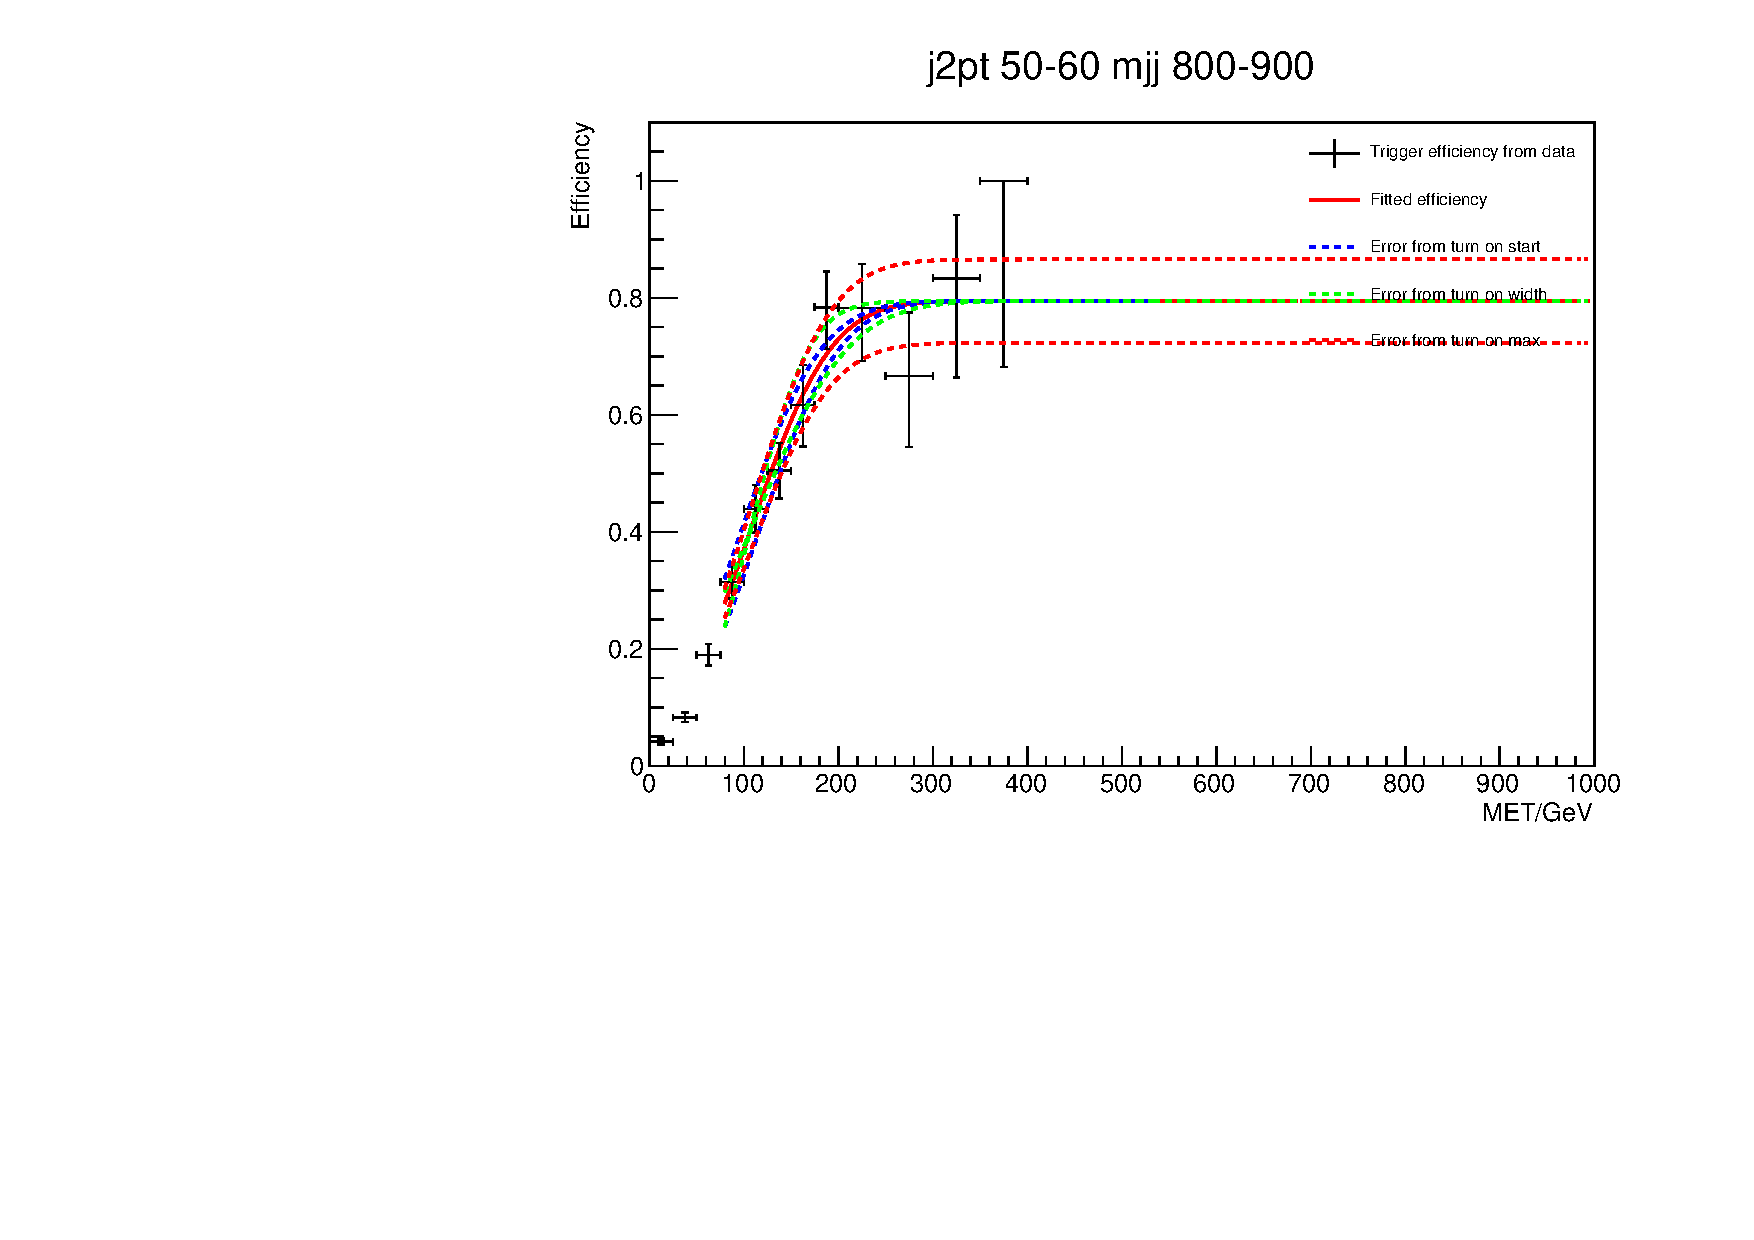
\includegraphics[width=.6\largefigwidth]{plots/parked/trigfitplots/hData_MET_1D_33BC.pdf}
    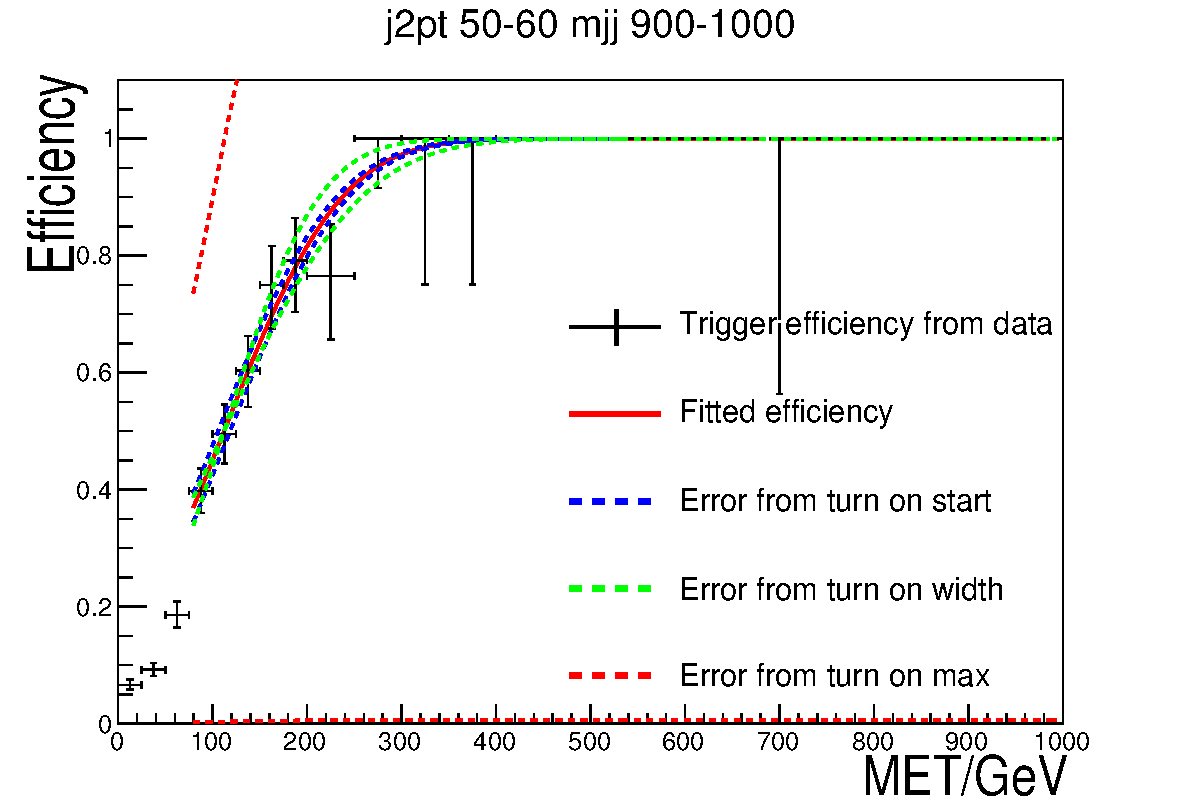
\includegraphics[width=.6\largefigwidth]{plots/parked/trigfitplots/hData_MET_1D_34BC.pdf}

    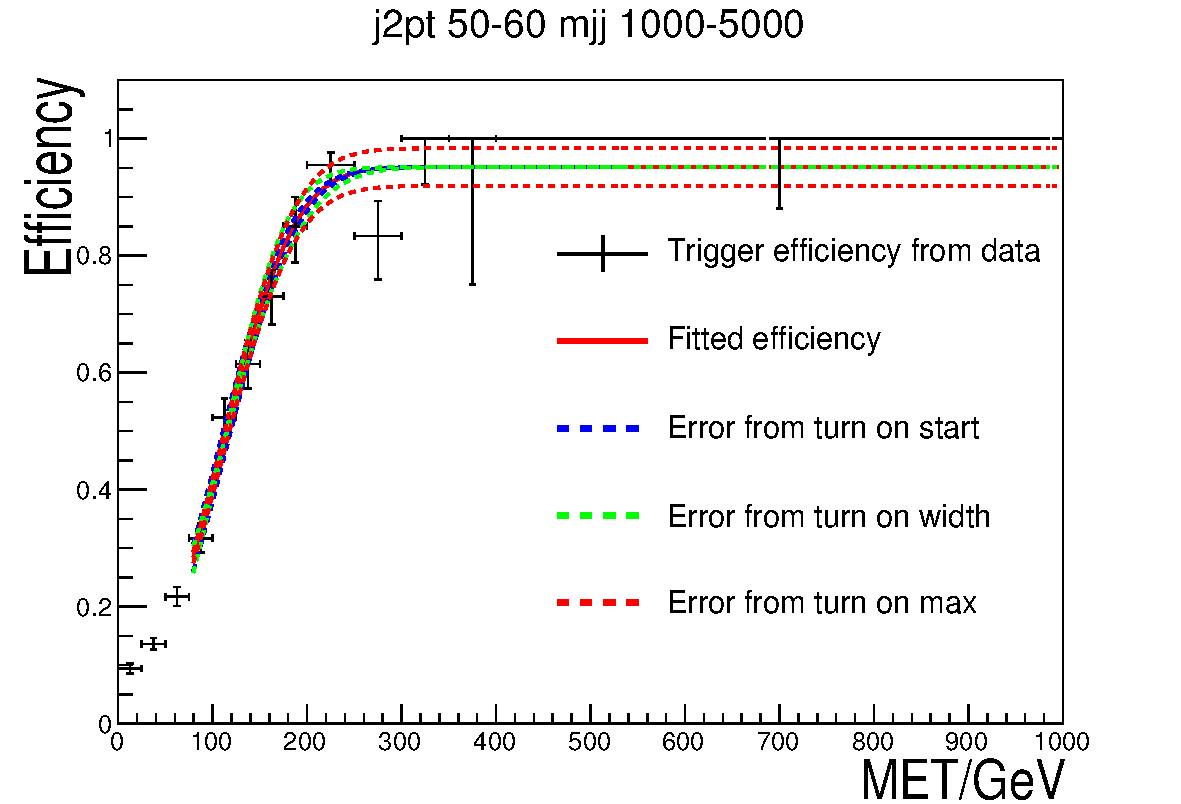
\includegraphics[width=.6\largefigwidth]{plots/parked/trigfitplots/hData_MET_1D_35BC.pdf}
    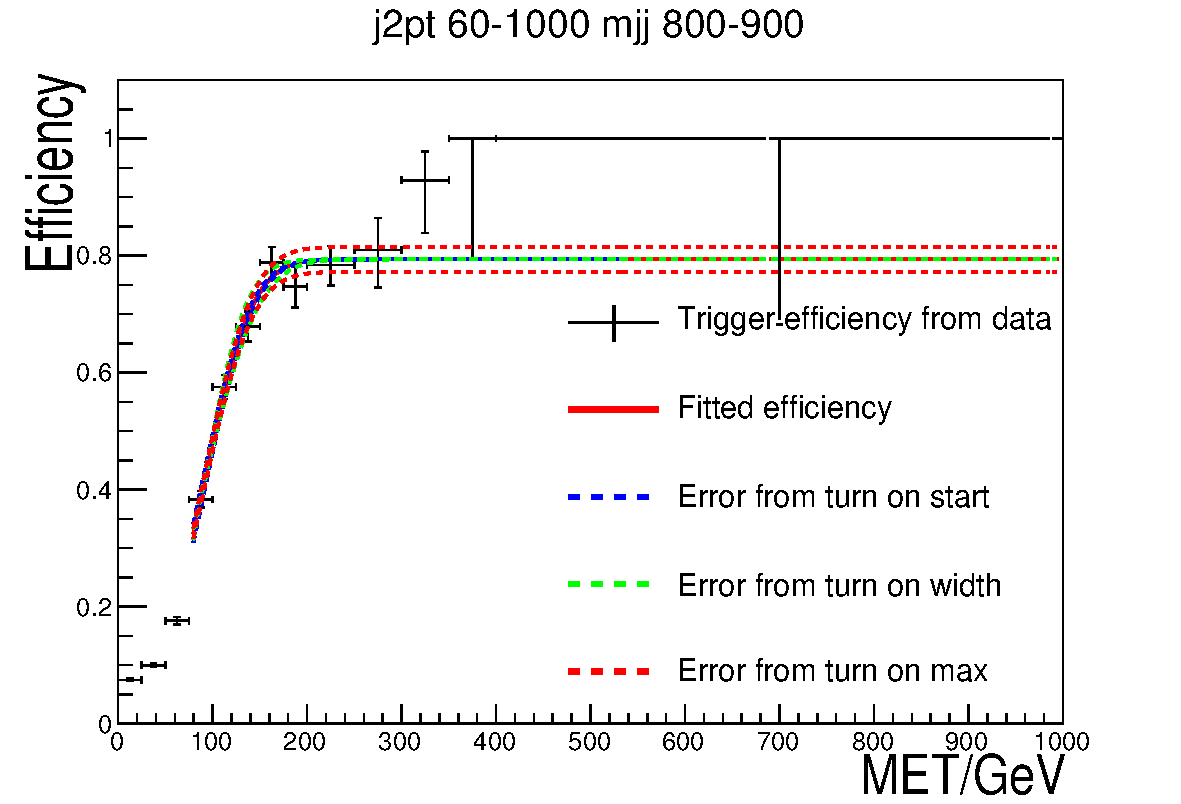
\includegraphics[width=.6\largefigwidth]{plots/parked/trigfitplots/hData_MET_1D_43BC.pdf}

    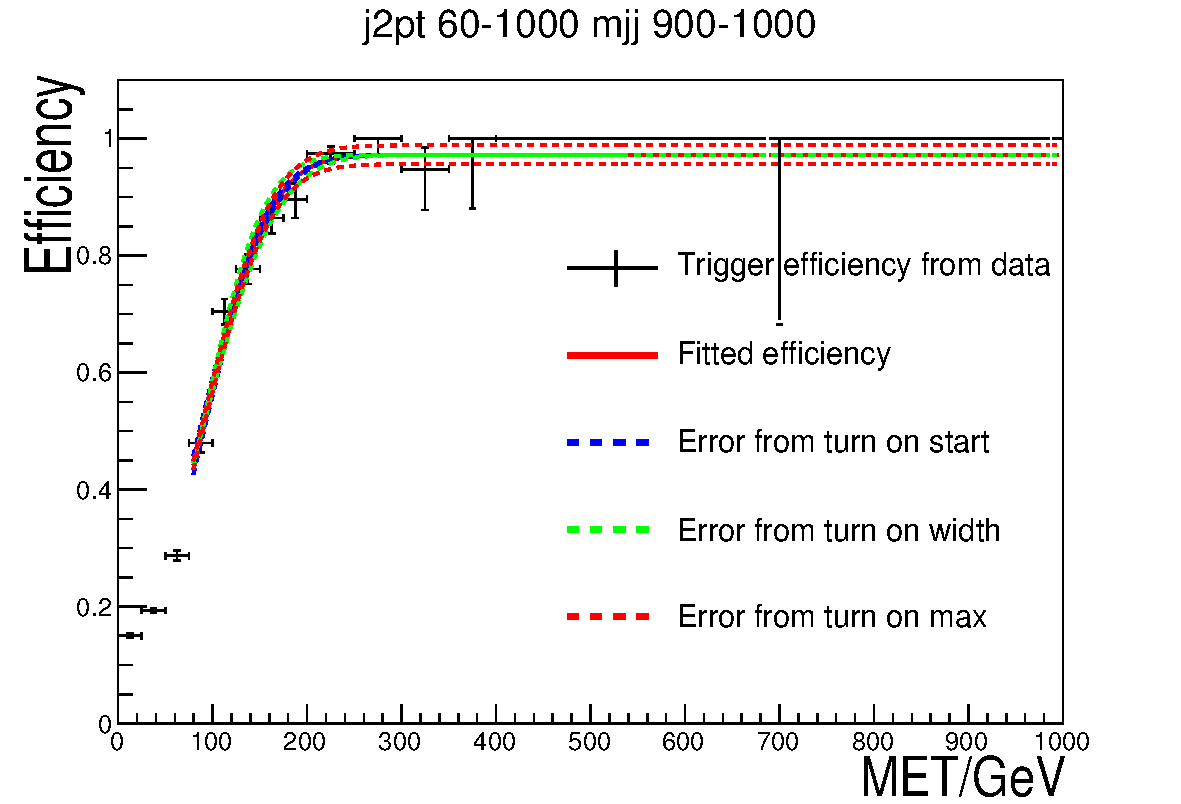
\includegraphics[width=.6\largefigwidth]{plots/parked/trigfitplots/hData_MET_1D_44BC.pdf}
    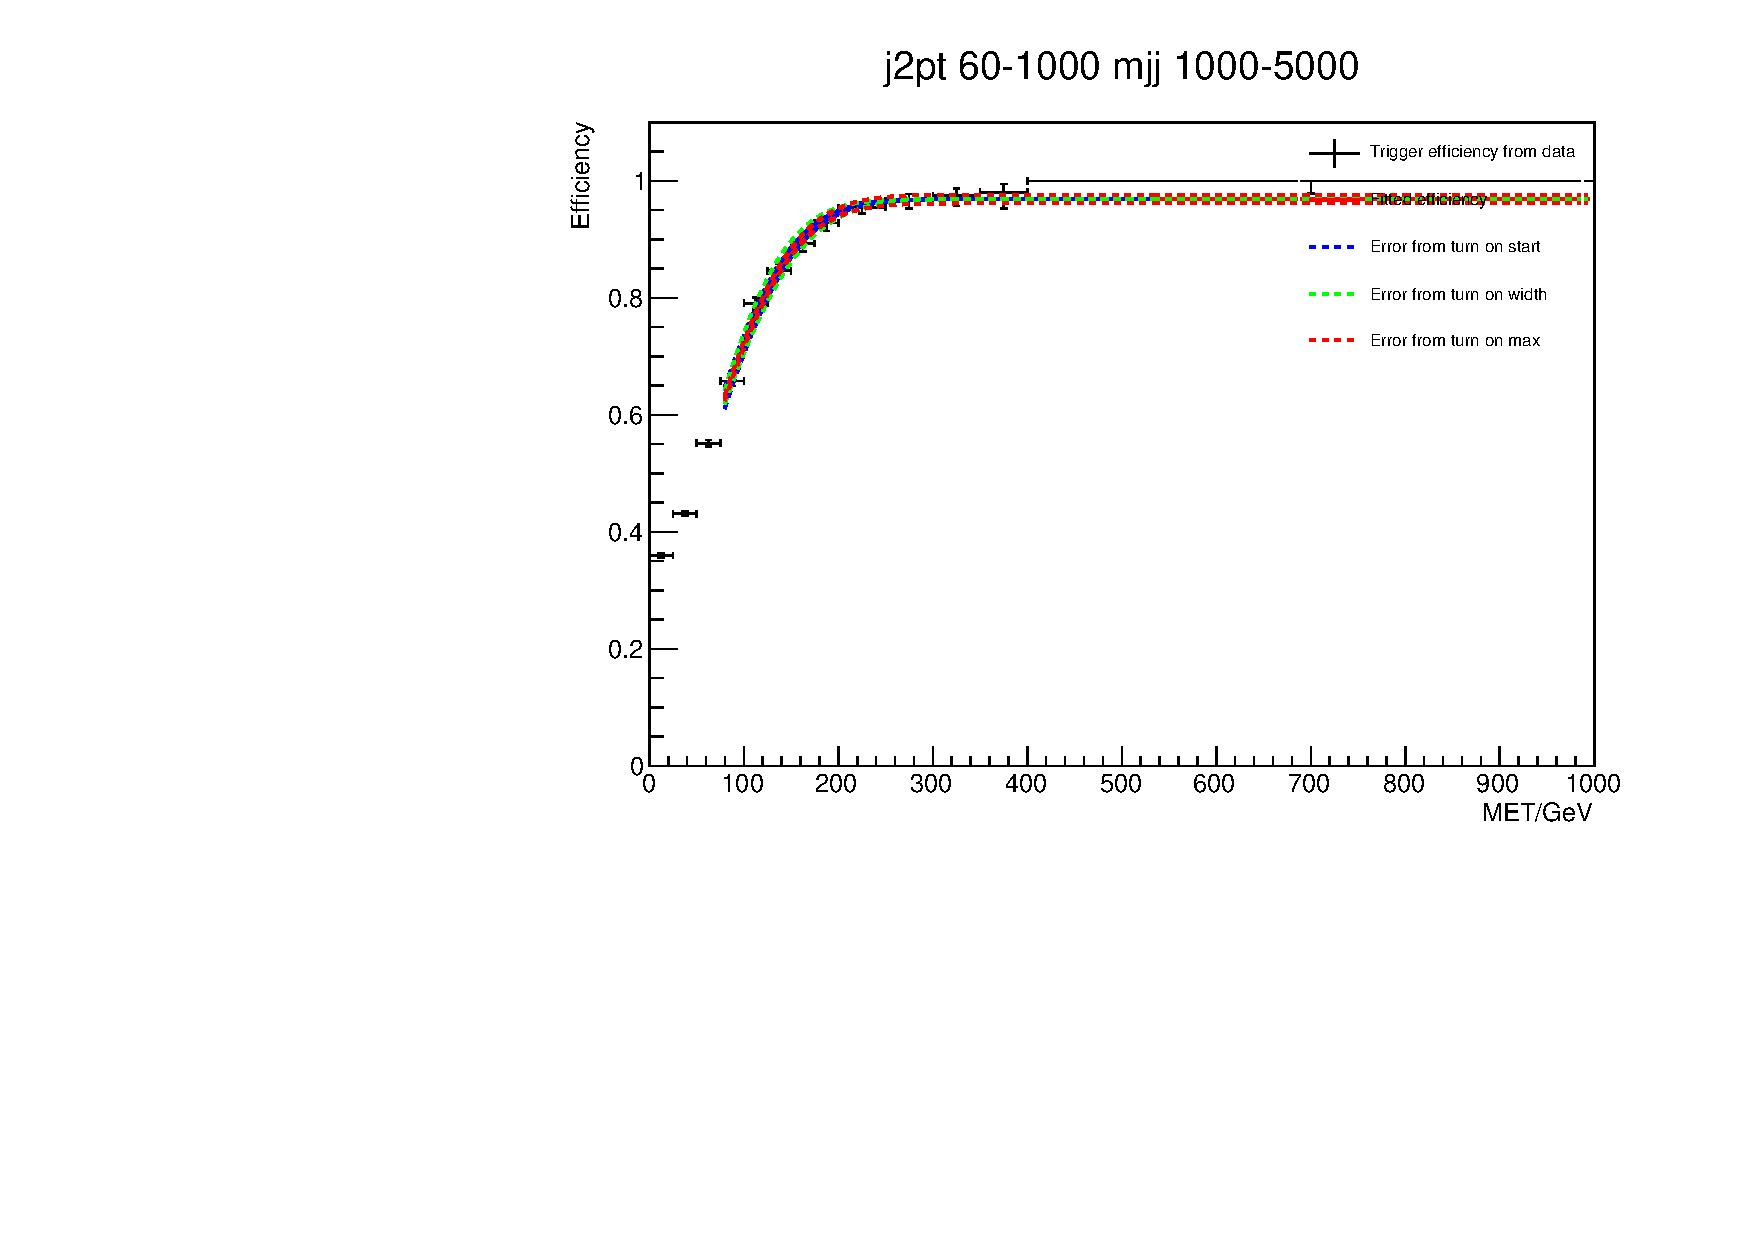
\includegraphics[width=.6\largefigwidth]{plots/parked/trigfitplots/hData_MET_1D_45BC.pdf}
    \caption{The measured efficiency of the trigger used in runs B and C as a function of MET in bins of dijet mass (mjj) and sub-leading jet $p_{T}$ (j2pt). The bin that each plot corresponds to is displayed at the top of the plot}
    \label{fig:trigfitplotsBC2}
  \end{center}
\end{figure}

\begin{figure}[h!]
  \begin{center}
    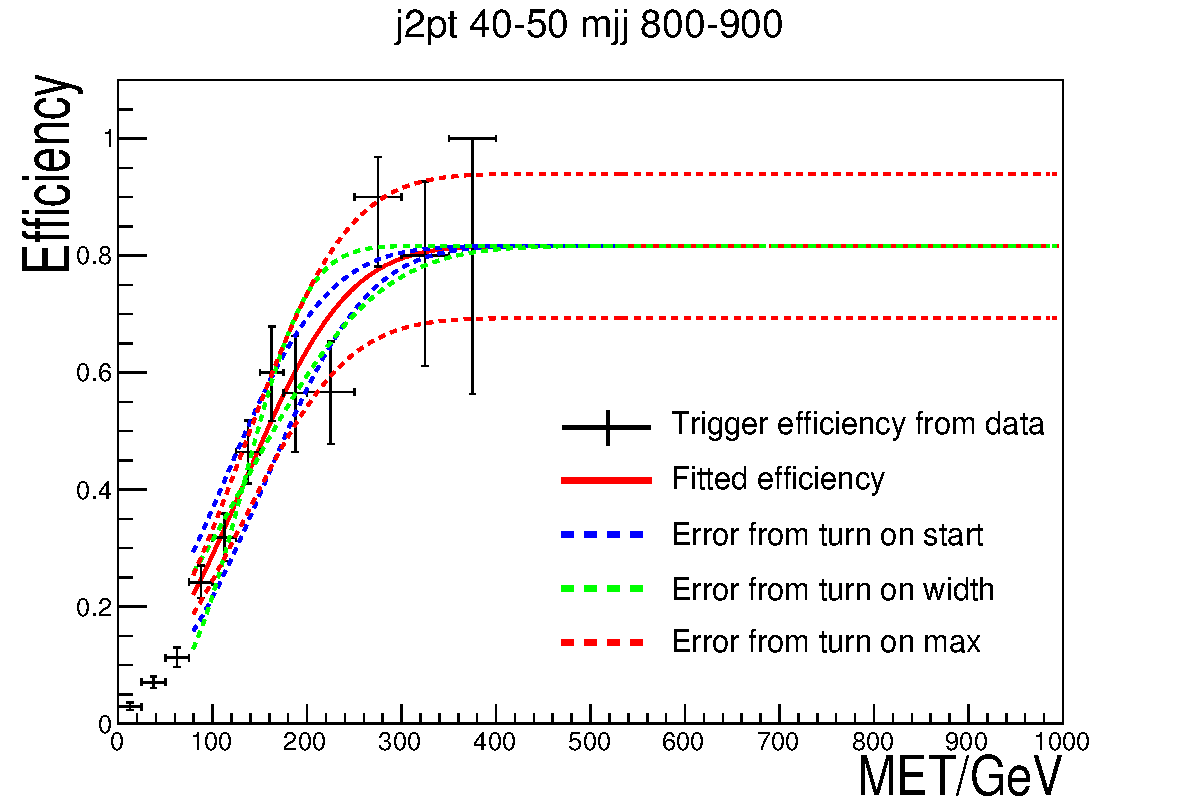
\includegraphics[width=.6\largefigwidth]{plots/parked/trigfitplots/hData_MET_1D_23D.pdf}
    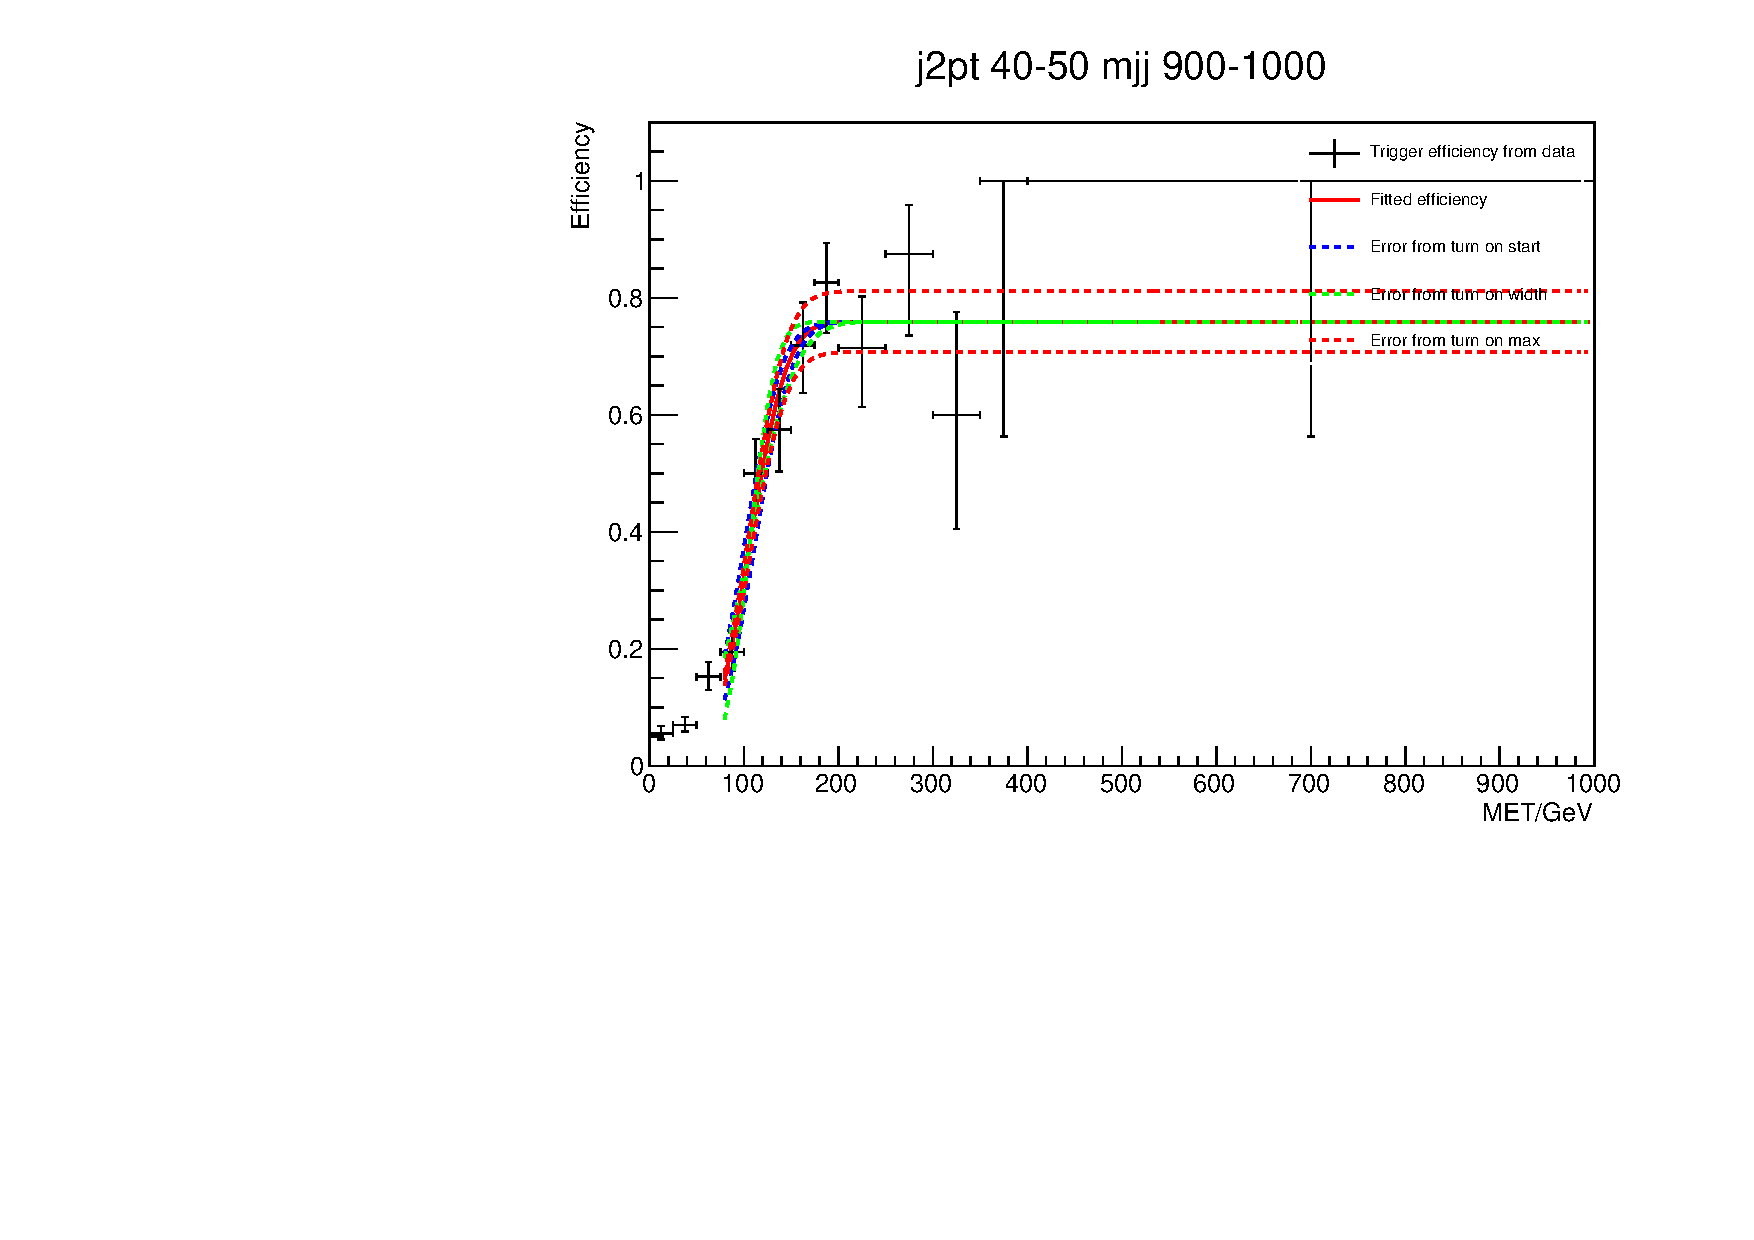
\includegraphics[width=.6\largefigwidth]{plots/parked/trigfitplots/hData_MET_1D_24D.pdf}

    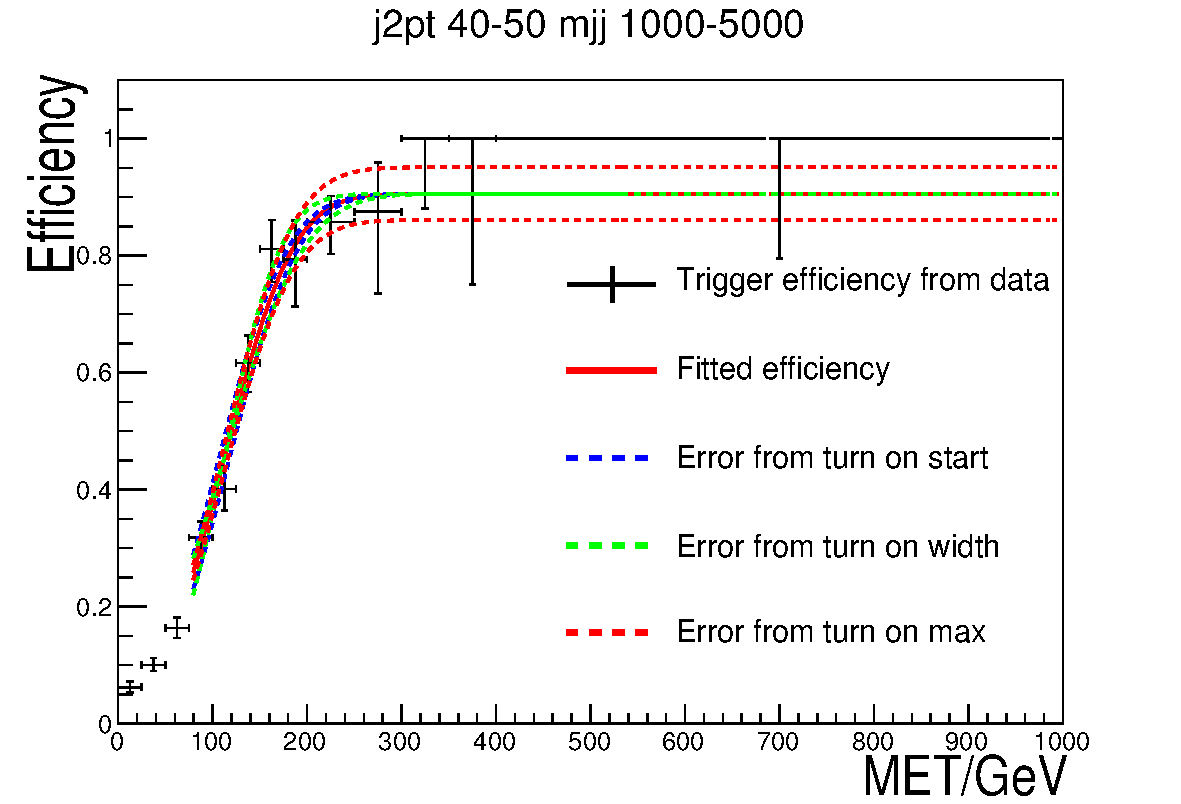
\includegraphics[width=.6\largefigwidth]{plots/parked/trigfitplots/hData_MET_1D_25D.pdf}
    \caption{The measured efficiency of the trigger used in run D as a function of MET in bins of dijet mass (mjj) and sub-leading jet $p_{T}$ (j2pt). The bin that each plot corresponds to is displayed at the top of the plot}
    \label{fig:trigfitplotsD1}
  \end{center}
\end{figure}

\begin{figure}
  \begin{center}
    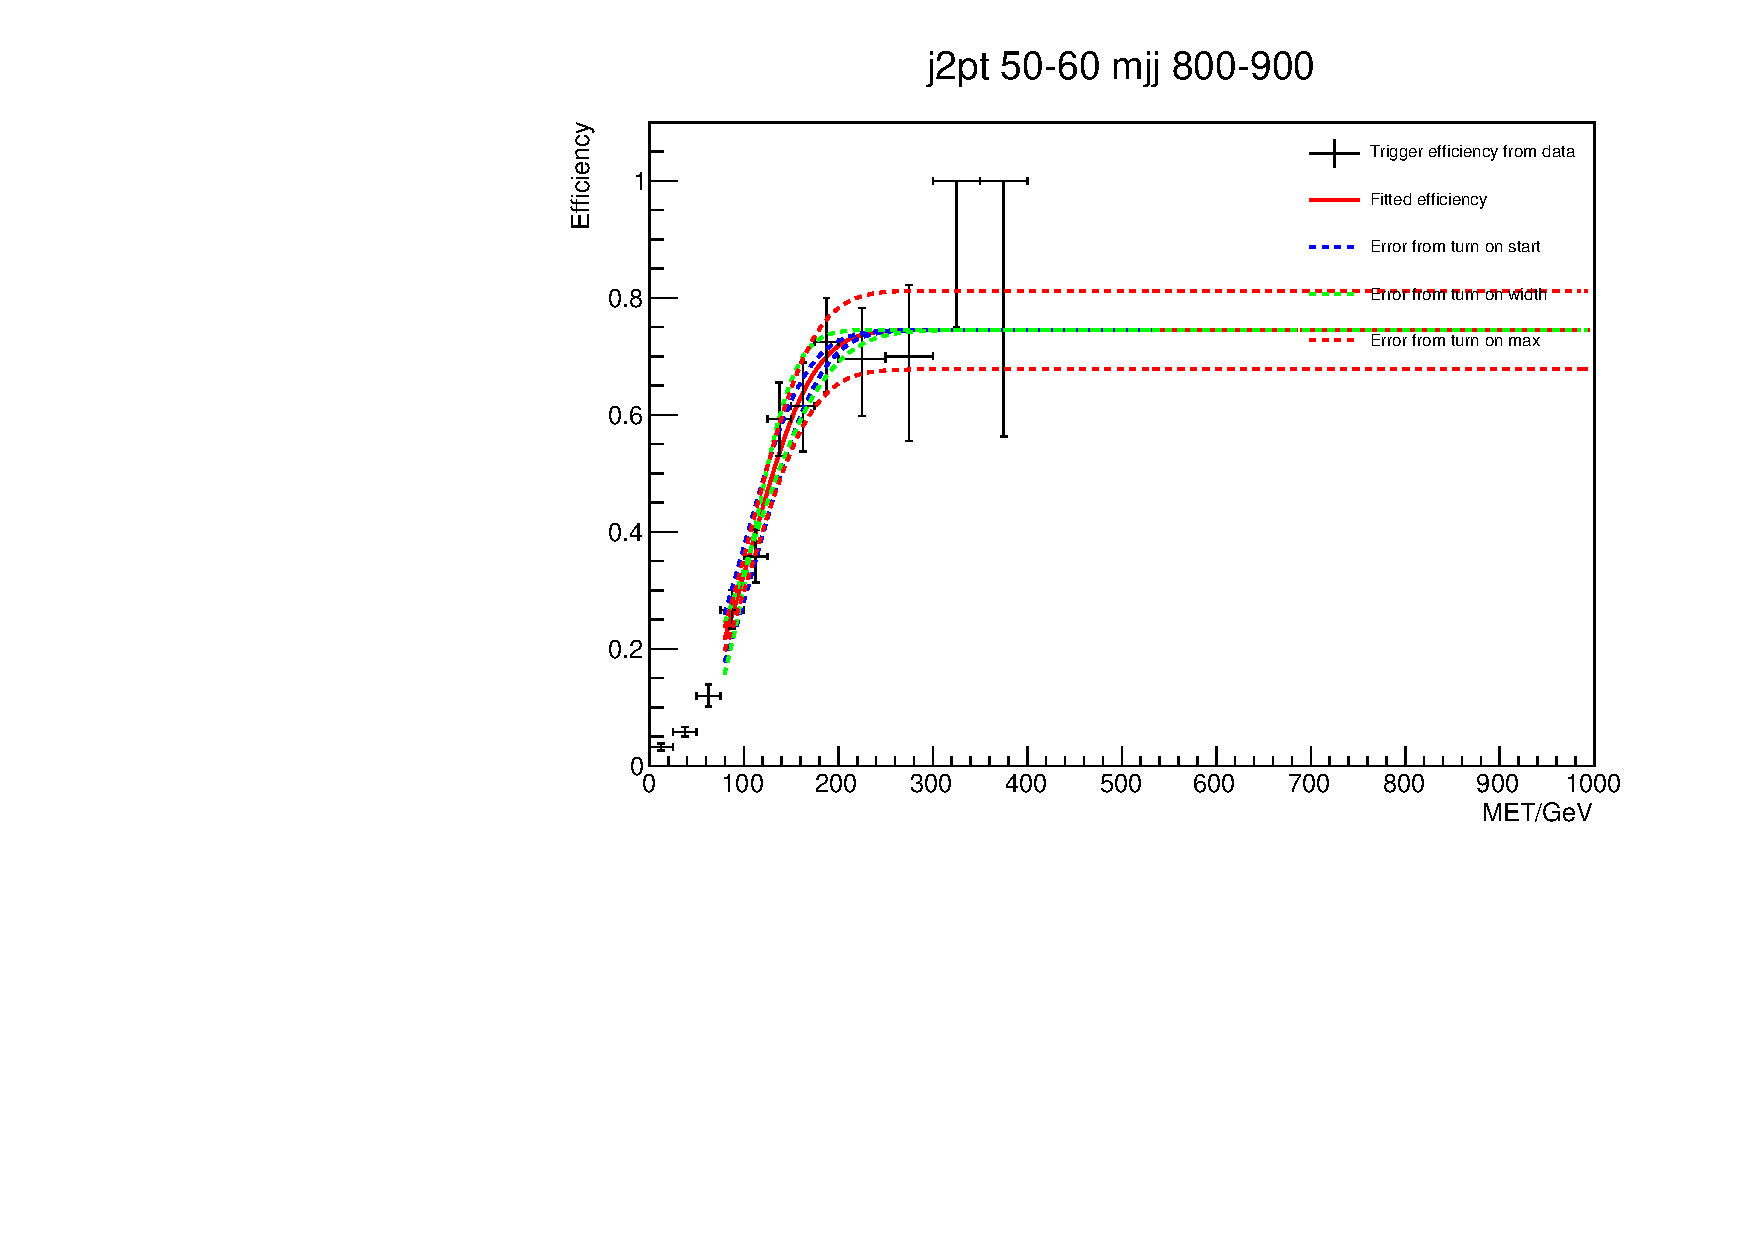
\includegraphics[width=.6\largefigwidth]{plots/parked/trigfitplots/hData_MET_1D_33D.pdf}
    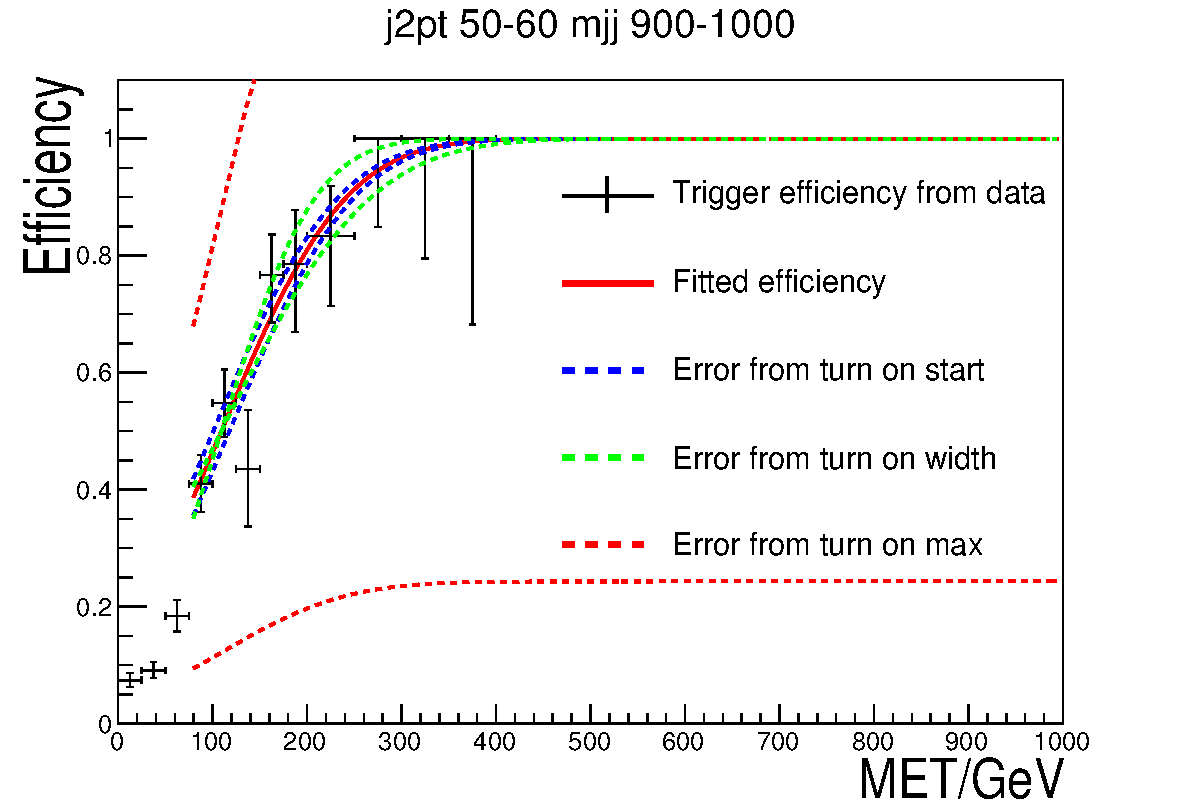
\includegraphics[width=.6\largefigwidth]{plots/parked/trigfitplots/hData_MET_1D_34D.pdf}

    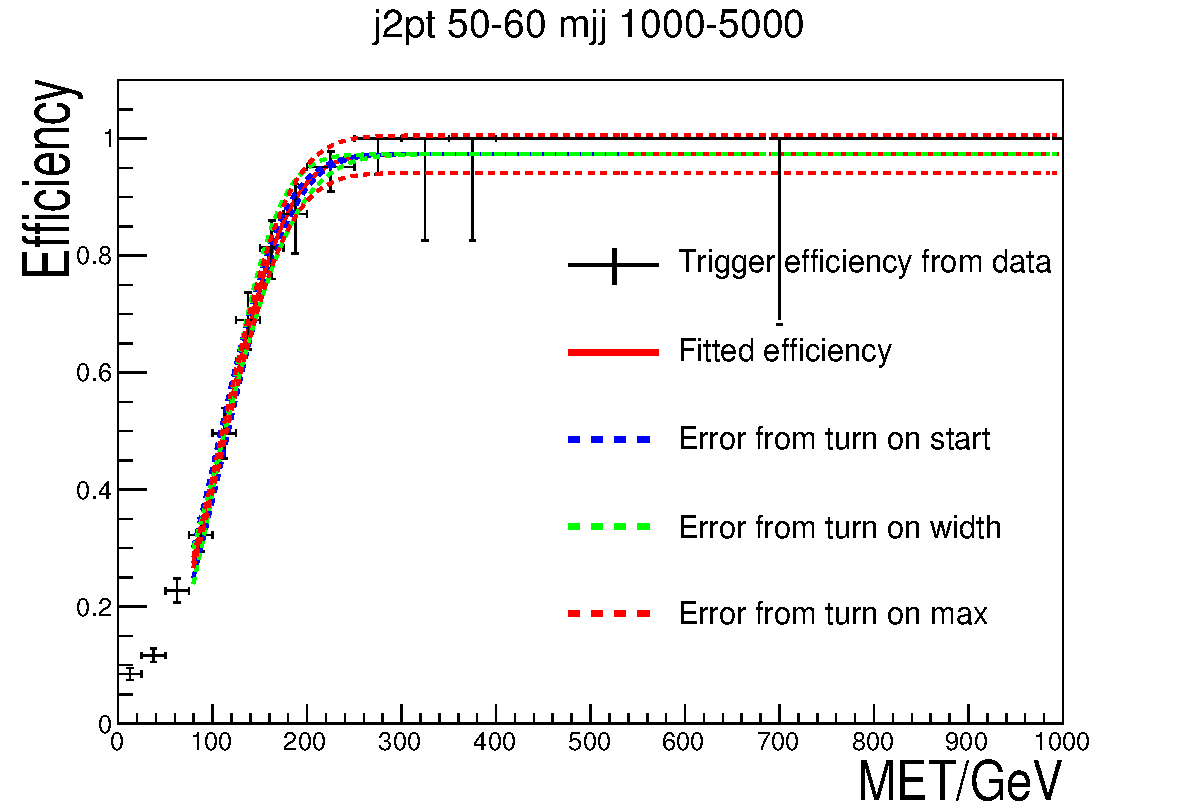
\includegraphics[width=.6\largefigwidth]{plots/parked/trigfitplots/hData_MET_1D_35D.pdf}
    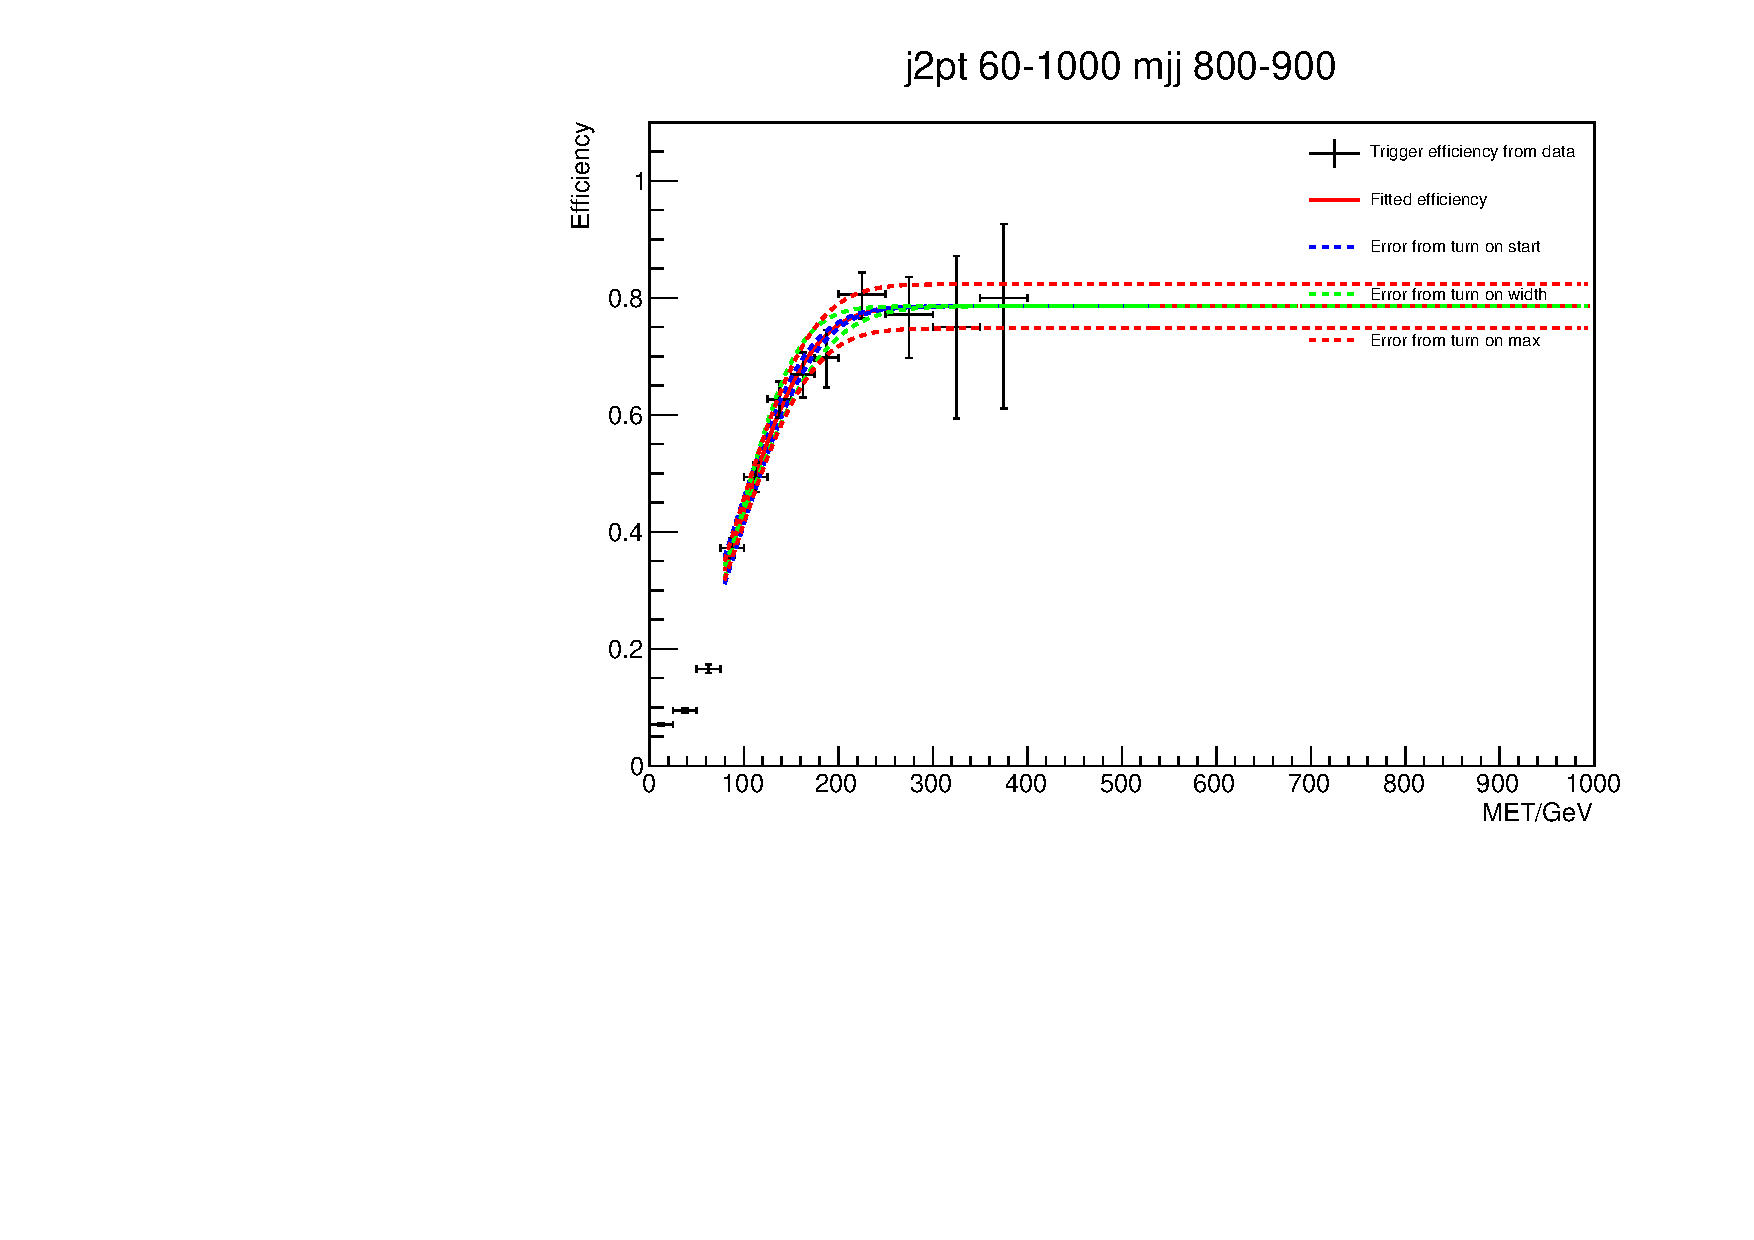
\includegraphics[width=.6\largefigwidth]{plots/parked/trigfitplots/hData_MET_1D_43D.pdf}

    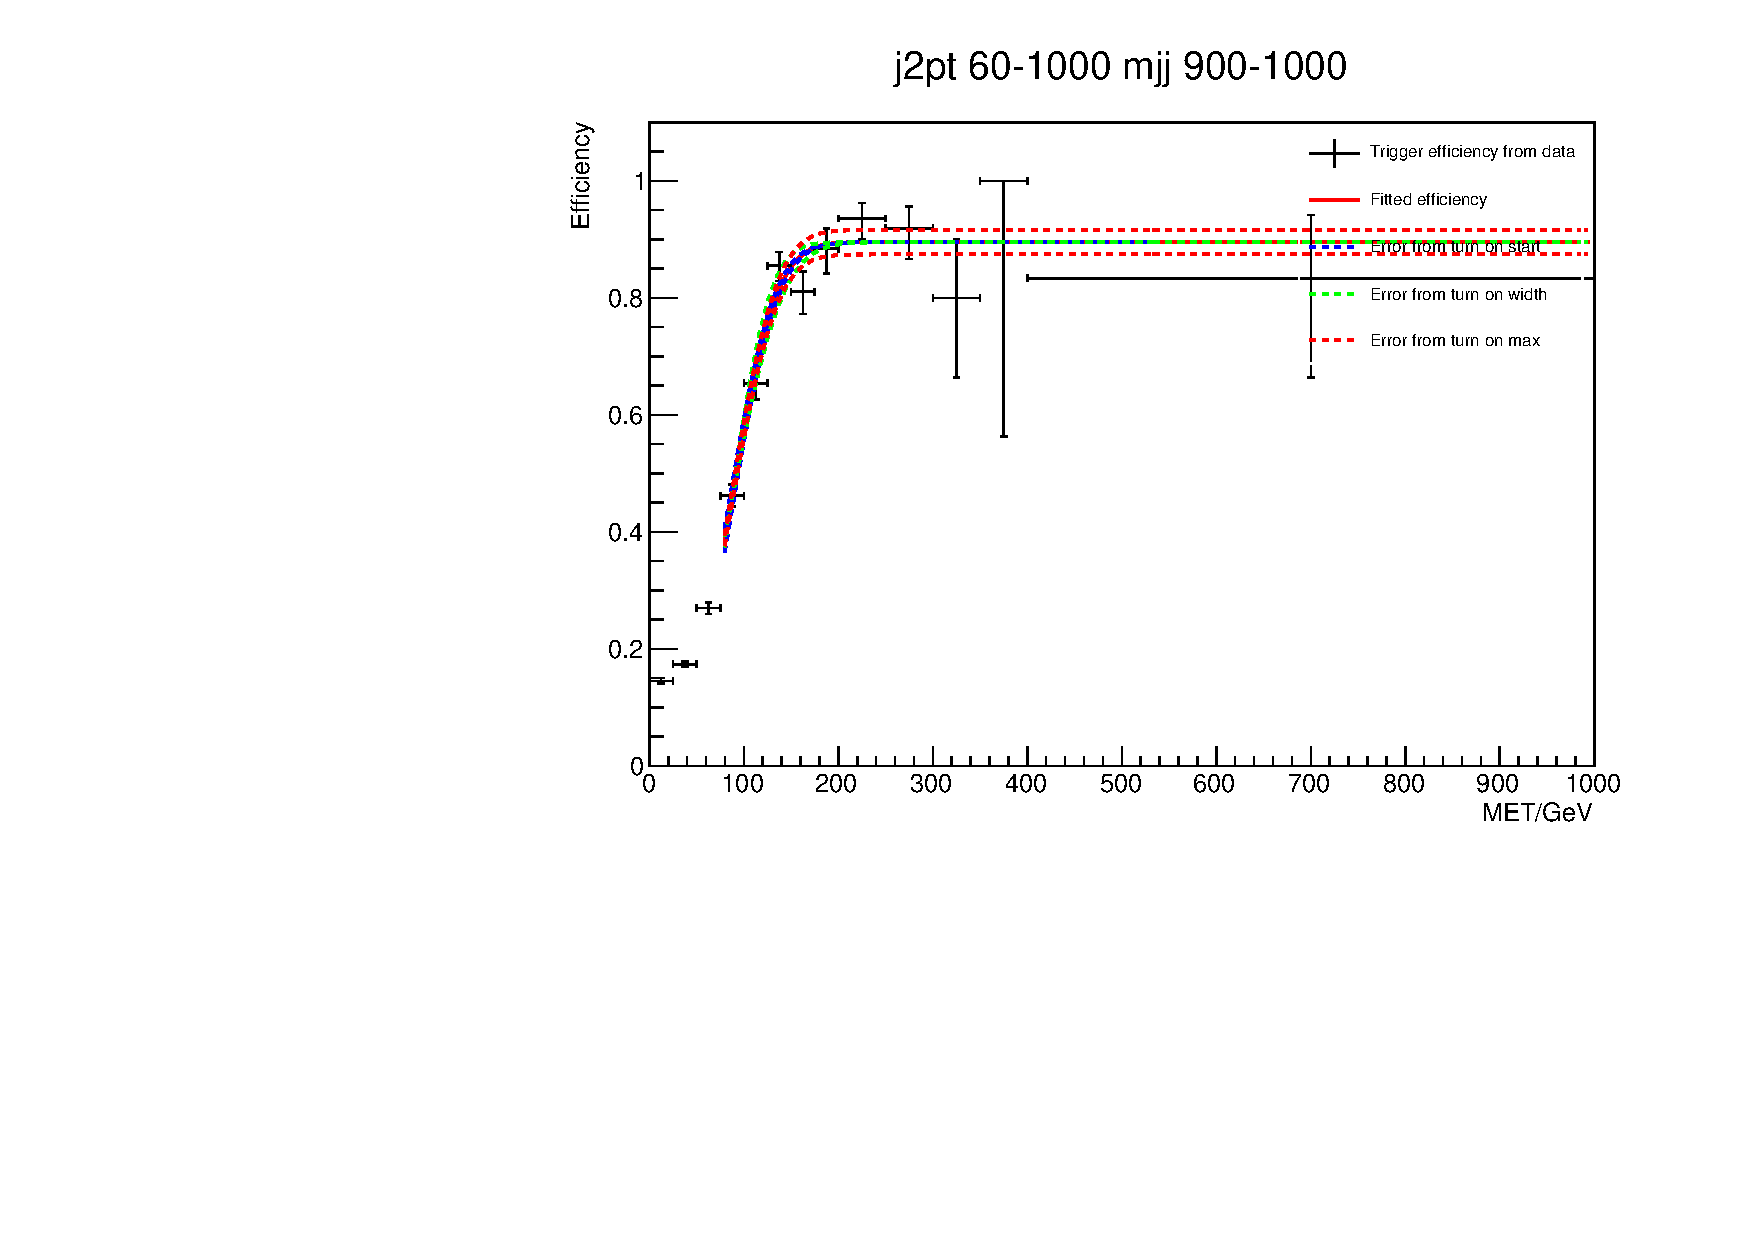
\includegraphics[width=.6\largefigwidth]{plots/parked/trigfitplots/hData_MET_1D_44D.pdf}
    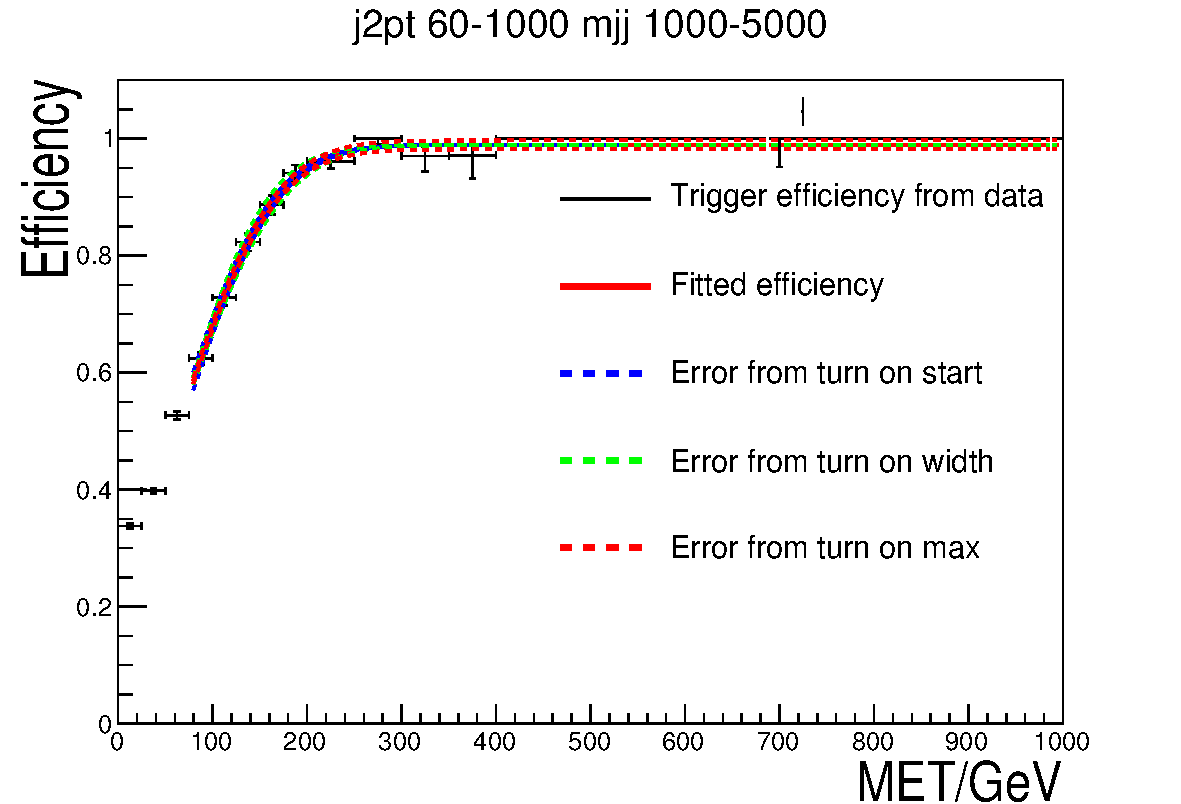
\includegraphics[width=.6\largefigwidth]{plots/parked/trigfitplots/hData_MET_1D_45D.pdf}
    \caption{The measured efficiency of the trigger used in run D as a function of MET in bins of dijet mass (mjj) and sub-leading jet $p_{T}$ (j2pt). The bin that each plot corresponds to is displayed at the top of the plot}
    \label{fig:trigfitplotsD2}
  \end{center}
\end{figure}
